% Options for packages loaded elsewhere
\PassOptionsToPackage{unicode}{hyperref}
\PassOptionsToPackage{hyphens}{url}
\PassOptionsToPackage{dvipsnames,svgnames,x11names}{xcolor}
%
\documentclass[
  a4paper,
]{article}

\usepackage{amsmath,amssymb}
\usepackage{iftex}
\ifPDFTeX
  \usepackage[T1]{fontenc}
  \usepackage[utf8]{inputenc}
  \usepackage{textcomp} % provide euro and other symbols
\else % if luatex or xetex
  \usepackage{unicode-math}
  \defaultfontfeatures{Scale=MatchLowercase}
  \defaultfontfeatures[\rmfamily]{Ligatures=TeX,Scale=1}
\fi
\usepackage{lmodern}
\ifPDFTeX\else  
    % xetex/luatex font selection
\fi
% Use upquote if available, for straight quotes in verbatim environments
\IfFileExists{upquote.sty}{\usepackage{upquote}}{}
\IfFileExists{microtype.sty}{% use microtype if available
  \usepackage[]{microtype}
  \UseMicrotypeSet[protrusion]{basicmath} % disable protrusion for tt fonts
}{}
\makeatletter
\@ifundefined{KOMAClassName}{% if non-KOMA class
  \IfFileExists{parskip.sty}{%
    \usepackage{parskip}
  }{% else
    \setlength{\parindent}{0pt}
    \setlength{\parskip}{6pt plus 2pt minus 1pt}}
}{% if KOMA class
  \KOMAoptions{parskip=half}}
\makeatother
\usepackage{xcolor}
\usepackage[top=2.54cm,right=2.54cm,bottom=2.54cm,left=2.54cm]{geometry}
\setlength{\emergencystretch}{3em} % prevent overfull lines
\setcounter{secnumdepth}{-\maxdimen} % remove section numbering
% Make \paragraph and \subparagraph free-standing
\ifx\paragraph\undefined\else
  \let\oldparagraph\paragraph
  \renewcommand{\paragraph}[1]{\oldparagraph{#1}\mbox{}}
\fi
\ifx\subparagraph\undefined\else
  \let\oldsubparagraph\subparagraph
  \renewcommand{\subparagraph}[1]{\oldsubparagraph{#1}\mbox{}}
\fi


\providecommand{\tightlist}{%
  \setlength{\itemsep}{0pt}\setlength{\parskip}{0pt}}\usepackage{longtable,booktabs,array}
\usepackage{calc} % for calculating minipage widths
% Correct order of tables after \paragraph or \subparagraph
\usepackage{etoolbox}
\makeatletter
\patchcmd\longtable{\par}{\if@noskipsec\mbox{}\fi\par}{}{}
\makeatother
% Allow footnotes in longtable head/foot
\IfFileExists{footnotehyper.sty}{\usepackage{footnotehyper}}{\usepackage{footnote}}
\makesavenoteenv{longtable}
\usepackage{graphicx}
\makeatletter
\def\maxwidth{\ifdim\Gin@nat@width>\linewidth\linewidth\else\Gin@nat@width\fi}
\def\maxheight{\ifdim\Gin@nat@height>\textheight\textheight\else\Gin@nat@height\fi}
\makeatother
% Scale images if necessary, so that they will not overflow the page
% margins by default, and it is still possible to overwrite the defaults
% using explicit options in \includegraphics[width, height, ...]{}
\setkeys{Gin}{width=\maxwidth,height=\maxheight,keepaspectratio}
% Set default figure placement to htbp
\makeatletter
\def\fps@figure{htbp}
\makeatother

% Preámbulo
\usepackage{comment} % Permite comentar secciones del código
\usepackage{marvosym} % Agrega símbolos adicionales
\usepackage{graphicx} % Permite insertar imágenes
\usepackage{mathptmx} % Fuente de texto matemática
\usepackage{amssymb} % Símbolos adicionales de matemáticas
\usepackage{lipsum} % Crea texto aleatorio
\usepackage{amsthm} % Teoremas y entornos de demostración
\usepackage{float} % Control de posiciones de figuras y tablas
\usepackage{rotating} % Rotación de elementos
\usepackage{multirow} % Celdas combinadas en tablas
\usepackage{tabularx} % Tablas con ancho de columna ajustable
\usepackage{mdframed} % Marcos alrededor de elementos flotantes

% Series de tiempo
\usepackage{booktabs}


% Configuración adicional

\makeatletter
\makeatother
\makeatletter
\makeatother
\makeatletter
\@ifpackageloaded{caption}{}{\usepackage{caption}}
\AtBeginDocument{%
\ifdefined\contentsname
  \renewcommand*\contentsname{Tabla de contenidos}
\else
  \newcommand\contentsname{Tabla de contenidos}
\fi
\ifdefined\listfigurename
  \renewcommand*\listfigurename{Listado de Figuras}
\else
  \newcommand\listfigurename{Listado de Figuras}
\fi
\ifdefined\listtablename
  \renewcommand*\listtablename{Listado de Tablas}
\else
  \newcommand\listtablename{Listado de Tablas}
\fi
\ifdefined\figurename
  \renewcommand*\figurename{Figura}
\else
  \newcommand\figurename{Figura}
\fi
\ifdefined\tablename
  \renewcommand*\tablename{Tabla}
\else
  \newcommand\tablename{Tabla}
\fi
}
\@ifpackageloaded{float}{}{\usepackage{float}}
\floatstyle{ruled}
\@ifundefined{c@chapter}{\newfloat{codelisting}{h}{lop}}{\newfloat{codelisting}{h}{lop}[chapter]}
\floatname{codelisting}{Listado}
\newcommand*\listoflistings{\listof{codelisting}{Listado de Listados}}
\makeatother
\makeatletter
\@ifpackageloaded{caption}{}{\usepackage{caption}}
\@ifpackageloaded{subcaption}{}{\usepackage{subcaption}}
\makeatother
\makeatletter
\@ifpackageloaded{tcolorbox}{}{\usepackage[skins,breakable]{tcolorbox}}
\makeatother
\makeatletter
\@ifundefined{shadecolor}{\definecolor{shadecolor}{rgb}{.97, .97, .97}}
\makeatother
\makeatletter
\makeatother
\makeatletter
\makeatother
\ifLuaTeX
\usepackage[bidi=basic]{babel}
\else
\usepackage[bidi=default]{babel}
\fi
\babelprovide[main,import]{spanish}
% get rid of language-specific shorthands (see #6817):
\let\LanguageShortHands\languageshorthands
\def\languageshorthands#1{}
\ifLuaTeX
  \usepackage{selnolig}  % disable illegal ligatures
\fi
\usepackage[]{biblatex}
\addbibresource{../../../../references.bib}
\IfFileExists{bookmark.sty}{\usepackage{bookmark}}{\usepackage{hyperref}}
\IfFileExists{xurl.sty}{\usepackage{xurl}}{} % add URL line breaks if available
\urlstyle{same} % disable monospaced font for URLs
\hypersetup{
  pdftitle={Notas de Clase Series de Tiempo},
  pdfauthor={Edison Achalma},
  pdflang={es},
  colorlinks=true,
  linkcolor={blue},
  filecolor={Maroon},
  citecolor={Blue},
  urlcolor={Blue},
  pdfcreator={LaTeX via pandoc}}

\title{Notas de Clase Series de Tiempo}
\usepackage{etoolbox}
\makeatletter
\providecommand{\subtitle}[1]{% add subtitle to \maketitle
  \apptocmd{\@title}{\par {\large #1 \par}}{}{}
}
\makeatother
\subtitle{Descubre cómo seleccionar hardware, descargar la imagen ISO y
preparar los medios de instalación. Exploraremos opciones para probar o
instalar Linux en tu equipo.}
\author{Edison Achalma}
\date{2023-08-27}

\begin{document}
\maketitle
\ifdefined\Shaded\renewenvironment{Shaded}{\begin{tcolorbox}[boxrule=0pt, interior hidden, frame hidden, borderline west={3pt}{0pt}{shadecolor}, sharp corners, enhanced, breakable]}{\end{tcolorbox}}\fi

\hypertarget{procesos-estacionarios-univariados}{%
\section{Procesos estacionarios
univariados}\label{procesos-estacionarios-univariados}}

En este capítulo analizaremos el método o metodología de análisis de
series de tiempo propuesto por Box y Jenkins (1970). Los modelos
propuestos dentro de está metodología o conjunto de métodos se han
vuelto indispensables para efectos de realizar pronósticos de corto
plazo.

En este sentido, se analizarán los métodos más importantes en series de
tiempo: Autoregresivos (AR) y de Medias Móviles (MA). Asimismo, se
realizará un análisis de los procesos que resultan de la combinación de
ambos, conocida como ARMA, los cuales son más comúnmente usados para
realizar pronósticos.

\hypertarget{procesos-autoregresivos-ar}{%
\subsection{Procesos Autoregresivos
(AR)}\label{procesos-autoregresivos-ar}}

Los procesos autoregresivos tienen su origen en el trabajo de Cochrane y
Orcutt de 1949, mediante el cual analizaron los residuales de una
regresión clásica como un proceso autoregresivo. Puede consultarse el
apéndice para la discusión del modelo de regresión clásica.

\hypertarget{ar1}{%
\subsubsection{AR(1)}\label{ar1}}

Como primer caso analizaremos al proceso autoregresivo de primer orden,
\(AR(1)\), el cual podemos definir como una Ecuación Lineal en
Diferencia Estocástica de Primer Orden. Diremos que una Ecuación Lineal
en Diferencia de Primer Orden es estocástica si en su representación
analítica considera un componente estocástico como en la ecuación
(\ref{EDO_Est}) descrita a continuación:

\begin{equation}\protect\hypertarget{eq-EDO_Est}{}{
X_t = a_0 + a_1 X_{t-1} + U_t
}\label{eq-EDO_Est}\end{equation}

Donde \(a_0\) es un término constante, \(U_t\) es un proceso
estacionario, con media cero (0), una varianza finita y constante
(\(\sigma^2\)) y una covarianza que depende de la distancia entre \(t\)
y cualquier \(t-s\) (\(\gamma_s\))--que no depende de los valores
pasados o futuros de la variable--, \(X_0\) es el valor inicial de
\(X_t\). No obstante, en general vamos a asumir que la covarianza será
cero (0), por lo que tendremos un proceso puramente aleatorio.
Considerando la ecuación (\ref{EDO_Est} y un proceso de sustitución
sucesivo podemos establecer lo siguiente, empezando con \(X_1\):

\begin{eqnarray*}
    X_{1} & = & a_0 + a_1 X_{0} + U_{1}
\end{eqnarray*}

Para \(X_2\):

\begin{eqnarray*}
X_{2} & = & a_0 + a_1 X_{1} + U_{2} \\
    & = & a_0 + a_1 (a_0 + a_1 X_{0} + U_{1}) + U_{2} \\
    & = & a_0 + a_1 a_0 + a_1^2 X_{0} + a_1 U_{1} + U_{2}
\end{eqnarray*}

Para \(X_3\):

\begin{eqnarray*}
X_{3} & = & a_0 + \alpha X_{2} + U_{3} \\
    & = & a_0 + a_1 (a_0 + a_1 a_0 + a_1^2 X_{0} + a_1 U_{1} + U_{2}) + U_{3} \\
    & = & a_0 + a_1 a_0 + a_1^2 a_0 + a_1^3 X_{0} + a_1^2 U_{1} + a_1 U_{2} + U_{3}
\end{eqnarray*}

Así, para cualquier \(X_t\), \(t = 1, 2, 3, \ldots\), obtendríamos:

\begin{eqnarray}
X_{t} & = & a_0 + a_1 X_{t - 1} + U_{t} \nonumber \\
    & = & a_0 + a_1 (a_0 + a_1 a_0 + a_1^2 a_0 + \ldots + a_1^{t-2} a_0 + a_1^{t-1} X_{0} \nonumber \\
    &   & + a_1^{t-2} U_{1} + \ldots + a_1 U_{t - 2} + U_{t - 1}) + U_{t} \nonumber \\
    & = & a_0 + a_1 a_0 + a_1^2 a_0 + a_1^3 a_0 + \ldots + a_1^{t-1} a_0 + a_1^{t} X_{0} \nonumber \\
    &   & + a_1^{t-1} U_{1} + \ldots a_1^2 U_{t - 2} + a_1 U_{t - 1} + U_{t} \nonumber \\
    & = & (1 + a_1 + a_1^2 + a_1^3 + \ldots + a_1^{t-1}) a_0 + a_1^{t} X_{0} \nonumber \\
    &   & + a_1^{t-1} U_{1} + \ldots + a_1^2 U_{t - 2} + a_1 U_{t - 1} + U_{t}  \nonumber\\
    & = & \frac{1 - a_1^t}{1 - a_1} a_0 + a_1^{t} X_{0} + \sum^{t-1}_{j = 0} a_1^{j} U_{t - j} 
\end{eqnarray} \{\#eq-EDO\_S\_Sol\}

De esta forma en la ecuación (\ref{EDO_S_Sol}) observamos un proceso que
es explicado por dos partes: una que depende del tiempo y otra que
depende de un proceso estocástico. Asimismo, debe notarse que la
condición de convergencia es idéntica que en el caso de ecuaciones en
diferencia estudiadas al inicio del curso: \(\abs{a_1} < 1\), por lo que
cuando \(t \to \infty\), la expresión (\ref{EDO_S_Sol}) será la
siguiente:

\begin{equation}\protect\hypertarget{eq-EDO_S_LP}{}{
X_t = \frac{1}{1 - a_1} a_0 + \sum^{\infty}_{j = 0} a_1^{j} U_{t - j}
}\label{eq-EDO_S_LP}\end{equation}

Así, desaparece la parte dependiente del tiempo y únicamente prevalece
la parte que es dependiente del proceso estocástico. Esta es la solución
de largo plazo del proceso \(AR(1)\), la cual depende del proceso
estocástico. Notemos, además, que esta solución implica que la variable
o la serie de tiempo \(X_t\) es tambien un proceso estocástico que
hereda las propiedades de \(U_t\). Así, \(X_t\) es también un proceso
estocástico estacionario, como demostraremos más adelante.

Observemos que la ecuación (\ref{EDO_S_LP}) se puede reescribir si
consideramos la formulación que en la literatura se denomina como la
descomposición de Wold, en la cual se define que es posible asumir que
\(\psi_j = a_1^j\) y se considera el caso en el cual \(\abs{a_1} < 1\),
de esta forma tendremos que por ejemplo cuando:

\[
    \sum^{\infty}_{j = 0} \psi^2_j = \sum^{\infty}_{j = 0} a_1^{2j} = \frac{1}{1 - a_1^2} 
\]

Alternativamente y de forma similar a las ecuaciones en diferencia
estudiadas previamente podemos escribir el proceso \(AR(1)\) mediante el
uso del operador rezago como:

\begin{eqnarray}
    X_t & = & a_0 + a_1 L X_t + U_t \nonumber \\
    X_t - a_1 L X_t & = & a_0 + U_t \nonumber \\
    (1 - a_1 L) X_t & = & a_0 + U_t \nonumber \\
    X_t & = & \frac{a_0}{1 - a_1 L} + \frac{1}{1 - a_1 L} U_t
\end{eqnarray} \{\#eq-AR\_1\}

En esta última ecuación retomamos el siguiente término para reescribirlo
como:

\[
\frac{1}{1 - a_1 L} = 1 + a_1 L + a_1^2 L^2 + a_1^3 L^3 + \ldots 
\]

Tomando este resultado para sustituirlo en ecuación (\ref{AR_1}),
obtenemos la siguiente expresión:

\begin{eqnarray}
X_t & = & (1 + a_1 L + a_1^2 L^2 + a_1^3 L^3 + \ldots) a_0 + (1 + a_1 L + a_1^2 L^2 + a_1^3 L^3 + \ldots) U_t \nonumber \\
    & = & (1 + a_1 + a_1^2 + a_1^3 + \ldots) a_0 + U_t + a_1 U_{t-1} + a_1^2 U_{t-2} + a_1^3 U_{t-3} + \ldots \nonumber \\
    & = & \frac{a_0}{1 - a_1} + \sum^{\infty}_{j = 0} a_1^j U_{t-j}
\end{eqnarray} \{\#eq-AR1\_Sol\}

Donde la condición de convergencia y estabilidad del proceso descrito en
esta ecuación es que \(\abs{a_1} < 1\). Por lo que hemos demostrado que
mediante el uso del operador de rezago es posible llegar al mismo
resultado que obtuvimos mediante el procedimiento de sustituciones
iterativas.

La ecuación (\ref{AR1_Sol}) se puede interpretar como sigue. La solución
o trayectoria de equilibrio de un AR(1) se divide en dos partes. La
primera es una constante que depende de los valores de \(a_0\) y
\(a_1\). La segunda parte es la suma ponderada de las desviaciones o
errores observados y acumulados en el tiempo hasta el momento \(t\).

Ahora obtendremos los momentos que describen a la serie de tiempo cuando
se trata de un porceso \(AR(1)\). Para ello debemos obtener la media, la
varianza y las covarianzas de \(X_t\). Para los siguientes resultados
debemos recordar y tener en mente que si \(U_t\) es un proceso puramente
aleatorio, entonces:

\begin{enumerate}
\def\labelenumi{\arabic{enumi}.}
\tightlist
\item
  \(\mathbb{E}[U_t] = 0\) para todo \(t\)
\item
  \(Var[U_t] = \sigma^2\) para todo \(t\)
\item
  \(Cov[U_t, U_s] = 0\) para todo \(t \neq s\)
\end{enumerate}

Dicho lo anterior y partiendo de la ecuación (\ref{AR1_Sol}), el primer
momento o valor esperado de la serie de tiempo será el siguiente:

\begin{eqnarray}
\mathbb{E}[X_t] & = & \mathbb{E} \left[ \frac{a_0}{1 - a_1} + \sum^{\infty}_{j = 0} a_1^j U_{t-j} \right] \nonumber \\
    & = & \frac{a_0}{1 - a_1} + \sum^{\infty}_{j = 0} a_1^j \mathbb{E}[U_{t-j}] \nonumber \\
    & = & \frac{a_0}{1 - a_1} = \mu
\end{eqnarray} \{\#eq-AR1\_m1\}

Respecto de la varianza podemos escribir la siguiente expresión a partir
de la ecuación (\ref{AR1_Sol}):

\begin{eqnarray}
Var[X_t] & = & \mathbb{E}[(X_t - \mu)^2] \nonumber \\
    & = & \mathbb{E} \left[ \left( \frac{a_0}{1 - a_1} + \sum^{\infty}_{j = 0} a_1^j U_{t-j} - \frac{a_0}{1 - a_1} \right)^2 \right] \nonumber \\
    & = & \mathbb{E}[(U_{t} + a_1 U_{t-1} + a_1^2 U_{t-2} + a_1^3 U_{t-3} + \ldots)^2] \nonumber \\
    & = & \mathbb{E}[U^2_{t} + a_1^2 U^2_{t-1} + a_1^4 U^2_{t-2} + a_1^6 U^2_{t-3} + \ldots \nonumber \\
    &   & + 2 a_1 U_t U_{t-1} + 2 a_1^2 U_t U_{t-2} + \ldots] \nonumber \\
    & = & \mathbb{E}[U^2_{t}] + a_1^2 \mathbb{E}[U^2_{t-1}] + a_1^4 \mathbb{E}[U^2_{t-2}] + a_1^6 \mathbb{E}[U^2_{t-3}] + \ldots \nonumber \\
    & = & \sigma^2 + a_1^2 \sigma^2 + a_1^4 \sigma^2 + a_1^6 \sigma^2 + \ldots \nonumber \\
    & = & \sigma^2 (1 + a_1^2 + a_1^4 + a_1^6 + \ldots) \nonumber \\
    & = & \sigma^2 \frac{1}{1 - a_1^2} = \gamma(0)
\end{eqnarray} \{\#eq-AR1\_Var\}

Previo a analizar la covarianza de la serie recordemos que para el
proceso puramente aleatorio \(U_t\) su varianza y covarianza puede verse
como \(\mathbb{E}[U_t, U_s] = \sigma^2\), para \(t = s\), y
\(\mathbb{E}[U_t, U_s] = 0\), para cualquier otro caso, respectivamente.

Dicho lo anterior, partiendo de la ecuación (\ref{AR1_Sol}) la
covarianza de la serie estará dada por:

\begin{eqnarray}
Cov(X_t, X_{t-\tau}) & = & \mathbb{E}[(X_t - \mu)(X_{t-\tau} - \mu)] \nonumber \\
    & = & \mathbb{E} \left[ \left( \frac{a_0}{1 - a_1} + \sum^{\infty}_{j = 0} a_1^j U_{t-j} - \frac{a_0}{1 - a_1} \right) \right. \nonumber \\
    &   & \left. \times \left( \frac{a_0}{1 - a_1} + \sum^{\infty}_{j = 0} a_1^j U_{t-\tau-j} - \frac{a_0}{1 - a_1} \right) \right] \nonumber \\
    & = & a_1^{\tau} \mathbb{E}[U^2_{t-\tau} + a_1 U^2_{t-\tau-1} + a_1^2 U^2_{t-\tau-2} + a_1^3 U^2_{t-\tau-3} + \ldots] \nonumber \\
    & = & a_1^{\tau} \sigma^2 \frac{1}{1 - a_1^2} = \gamma(\tau)
\end{eqnarray} \{\#eq-AR1\_Cov\}

Notése que con estos resultados en las ecuaciones (\ref{AR1_Var}) y
(\ref{AR1_Cov}) podemos construir la función de autocorrelación teórica
como sigue:

\begin{eqnarray}
\rho(\tau) & = & \frac{\gamma(\tau)}{\gamma(0)} \nonumber \\
    & = & a_1^\tau
\end{eqnarray}

Donde \(\tau = 1, 2, 3, \ldots\) y \(\abs{a_1} < 1\). Este último
resultado significa que cuando el proceso autoregresivo es de orden 1
(es decir, AR(1)) la función de autocorrelación teóricamente es igual al
parámetro \(a_1\) elevado al número de rezagos considerados. No
obstante, note que esto no significa que la autocorrelación observada
sea como lo expresa en planteamiento anterior. Por el contrario, una
observación sencilla mostraría que la autocorrelación observada sería
ligeramente distinta a la autocorrelación teórica.

Ahora veámos algunos ejemplos. En el primer ejemplo simularemos una
serie y mostraremos el analísis de un proceso construído considerando un
proceso puramente aleatorio como componente
\(U_t\).\footnote{ El procedimiento e implementación del ejercicio está en el archivo R denominado Clase 4 del repositorio de GitHub.}
Por su parte, en un segundo ejemplo aplicaremos el análisis a una serie
de tiempo de una variable económica
observada.\footnote{ El procedimiento e implementación del ejercicio está en el archivo R denominado Clase 5 del repositorio de GitHub.}

Para el primer ejemplo consideremos un proceso dado por la forma de un
\(AR(1)\) como en la ecuación (\ref{AR_1}) cuya solución esta dada por
la ecuación (\ref{AR1_Sol}). En especifico, supongamos que el término o
componente estocástico \(U_t\) es una serie generada a partir de numeros
aleatorios de una función normal con media \(0\) y desviación estándar
\(4\). Los detalles del proceso simulado se muestra en las siguientes
gráficas.

La Figura \ref{G_AR_1_Real} ilustra el comportamiento que se debería
observar en una serie considerando el procedimiento iterativo de
construcción. Por su parte, la Figura \ref{G_AR_1_Teo} ilustra el
proceso o trayectoria de la solución de la serie de tiempo. Finalmente,
las Figuras \ref{G_AR_1_FACr} y \ref{G_AR_1_FACt} muestran el
correlograma calculado considerando una función de autocorrelación
aplicada al porceso real y una función de autocorrelación aplicada al
proceso teórico, respectivamente.

\begin{figure}
  \centering
    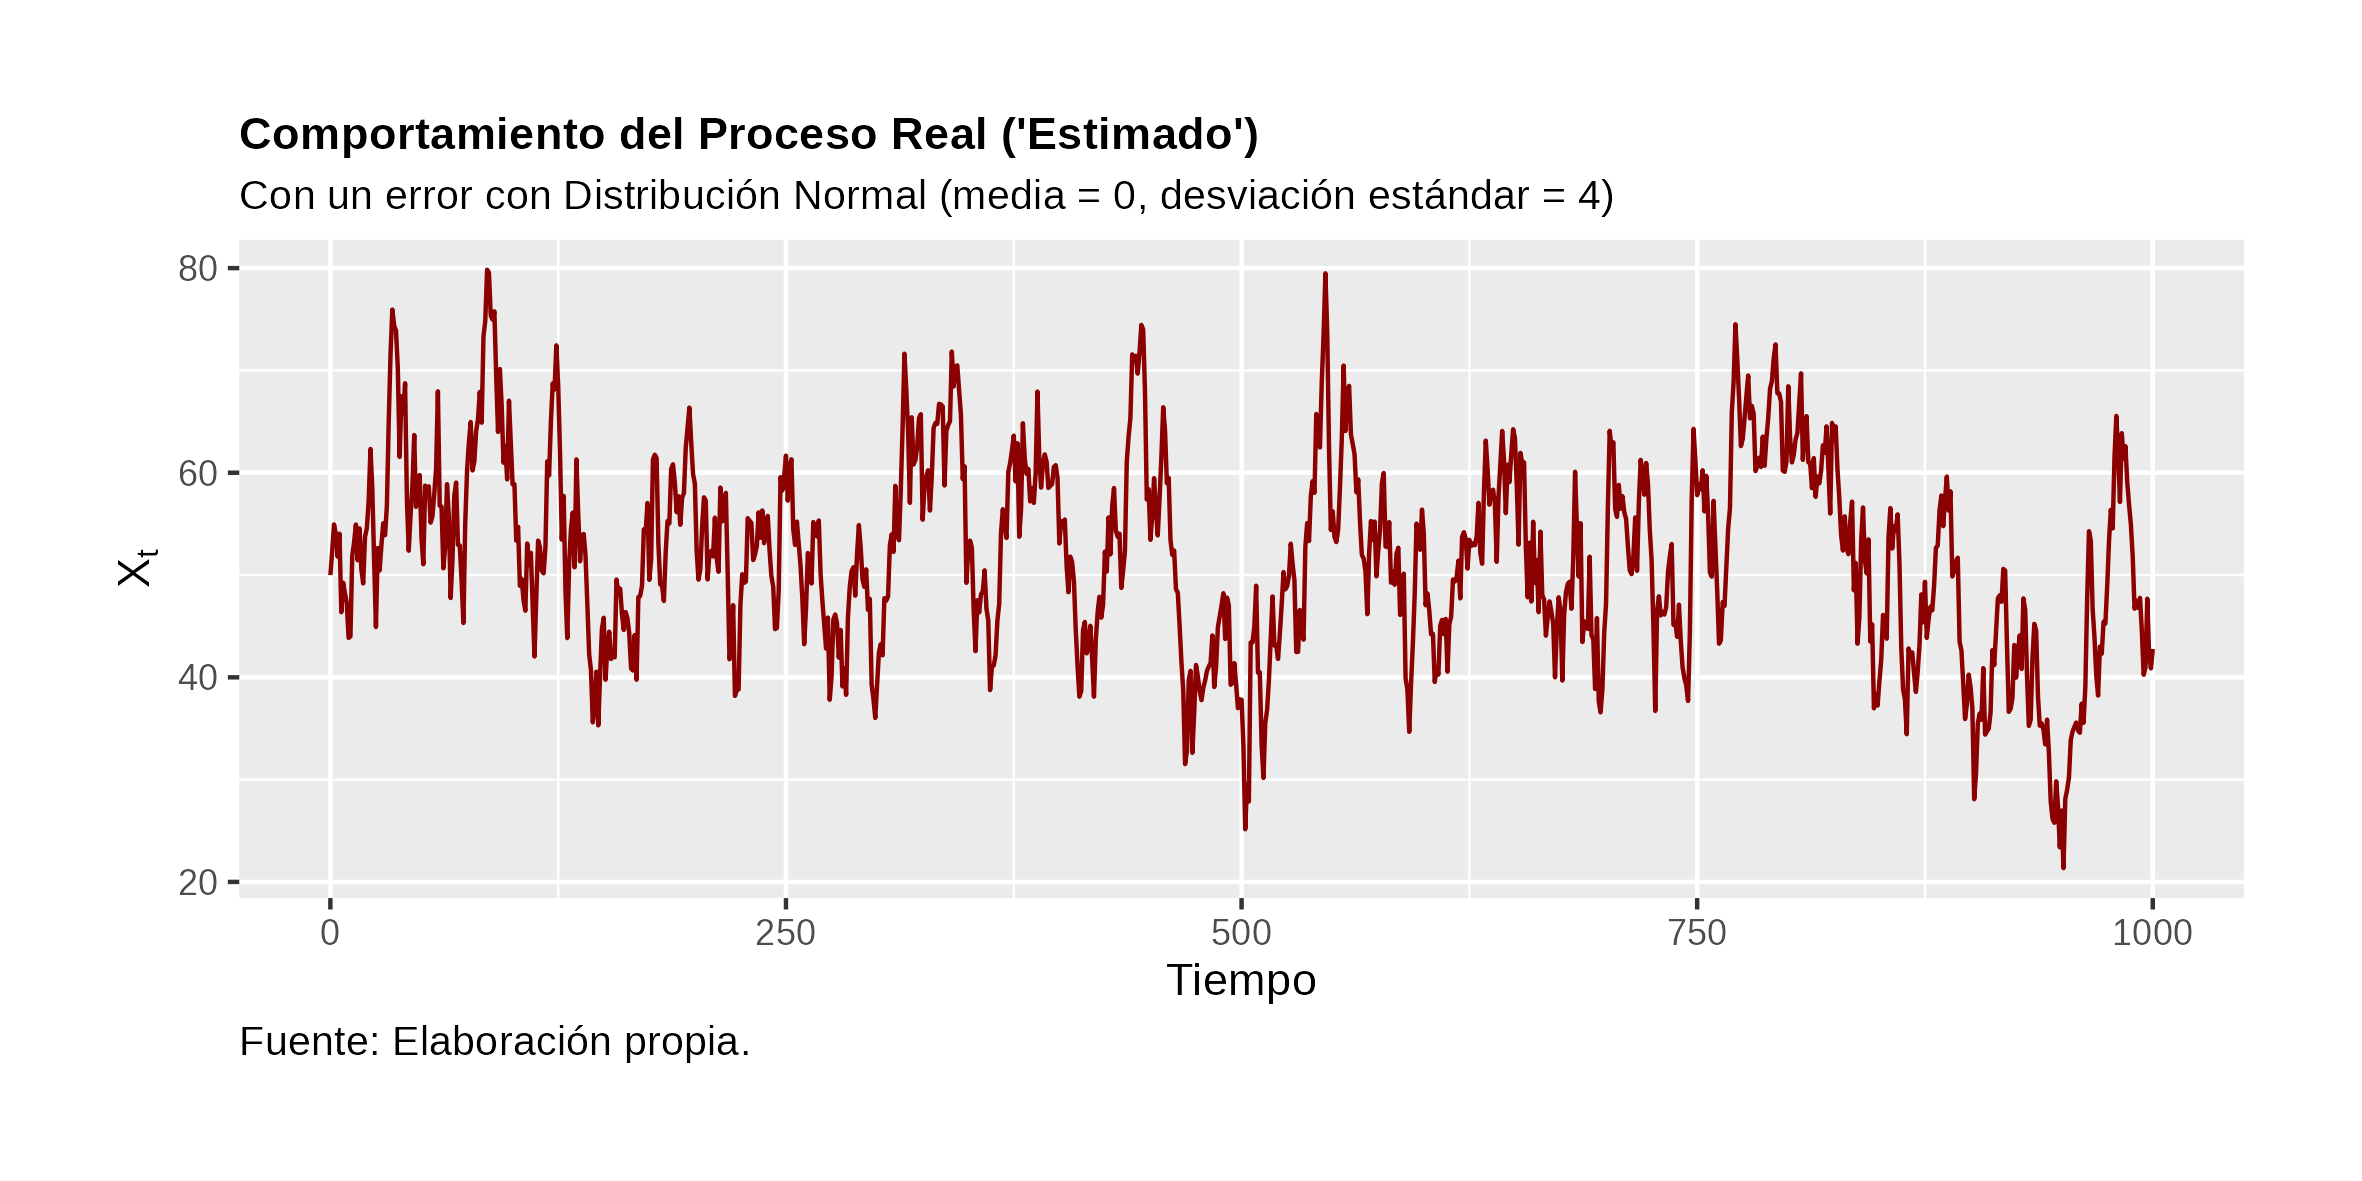
\includegraphics[width = 1.0 \textwidth]{G_AR_1_Real}
  \caption{AR(1) considerando $X_t = 5 + 0.9 X_{t-1} + U_t$; $X_0 = 50$, y que $U_t \sim \mathcal{N}(0, 4)$}
  \label{G_AR_1_Real}
\end{figure}

\begin{figure}
  \centering
    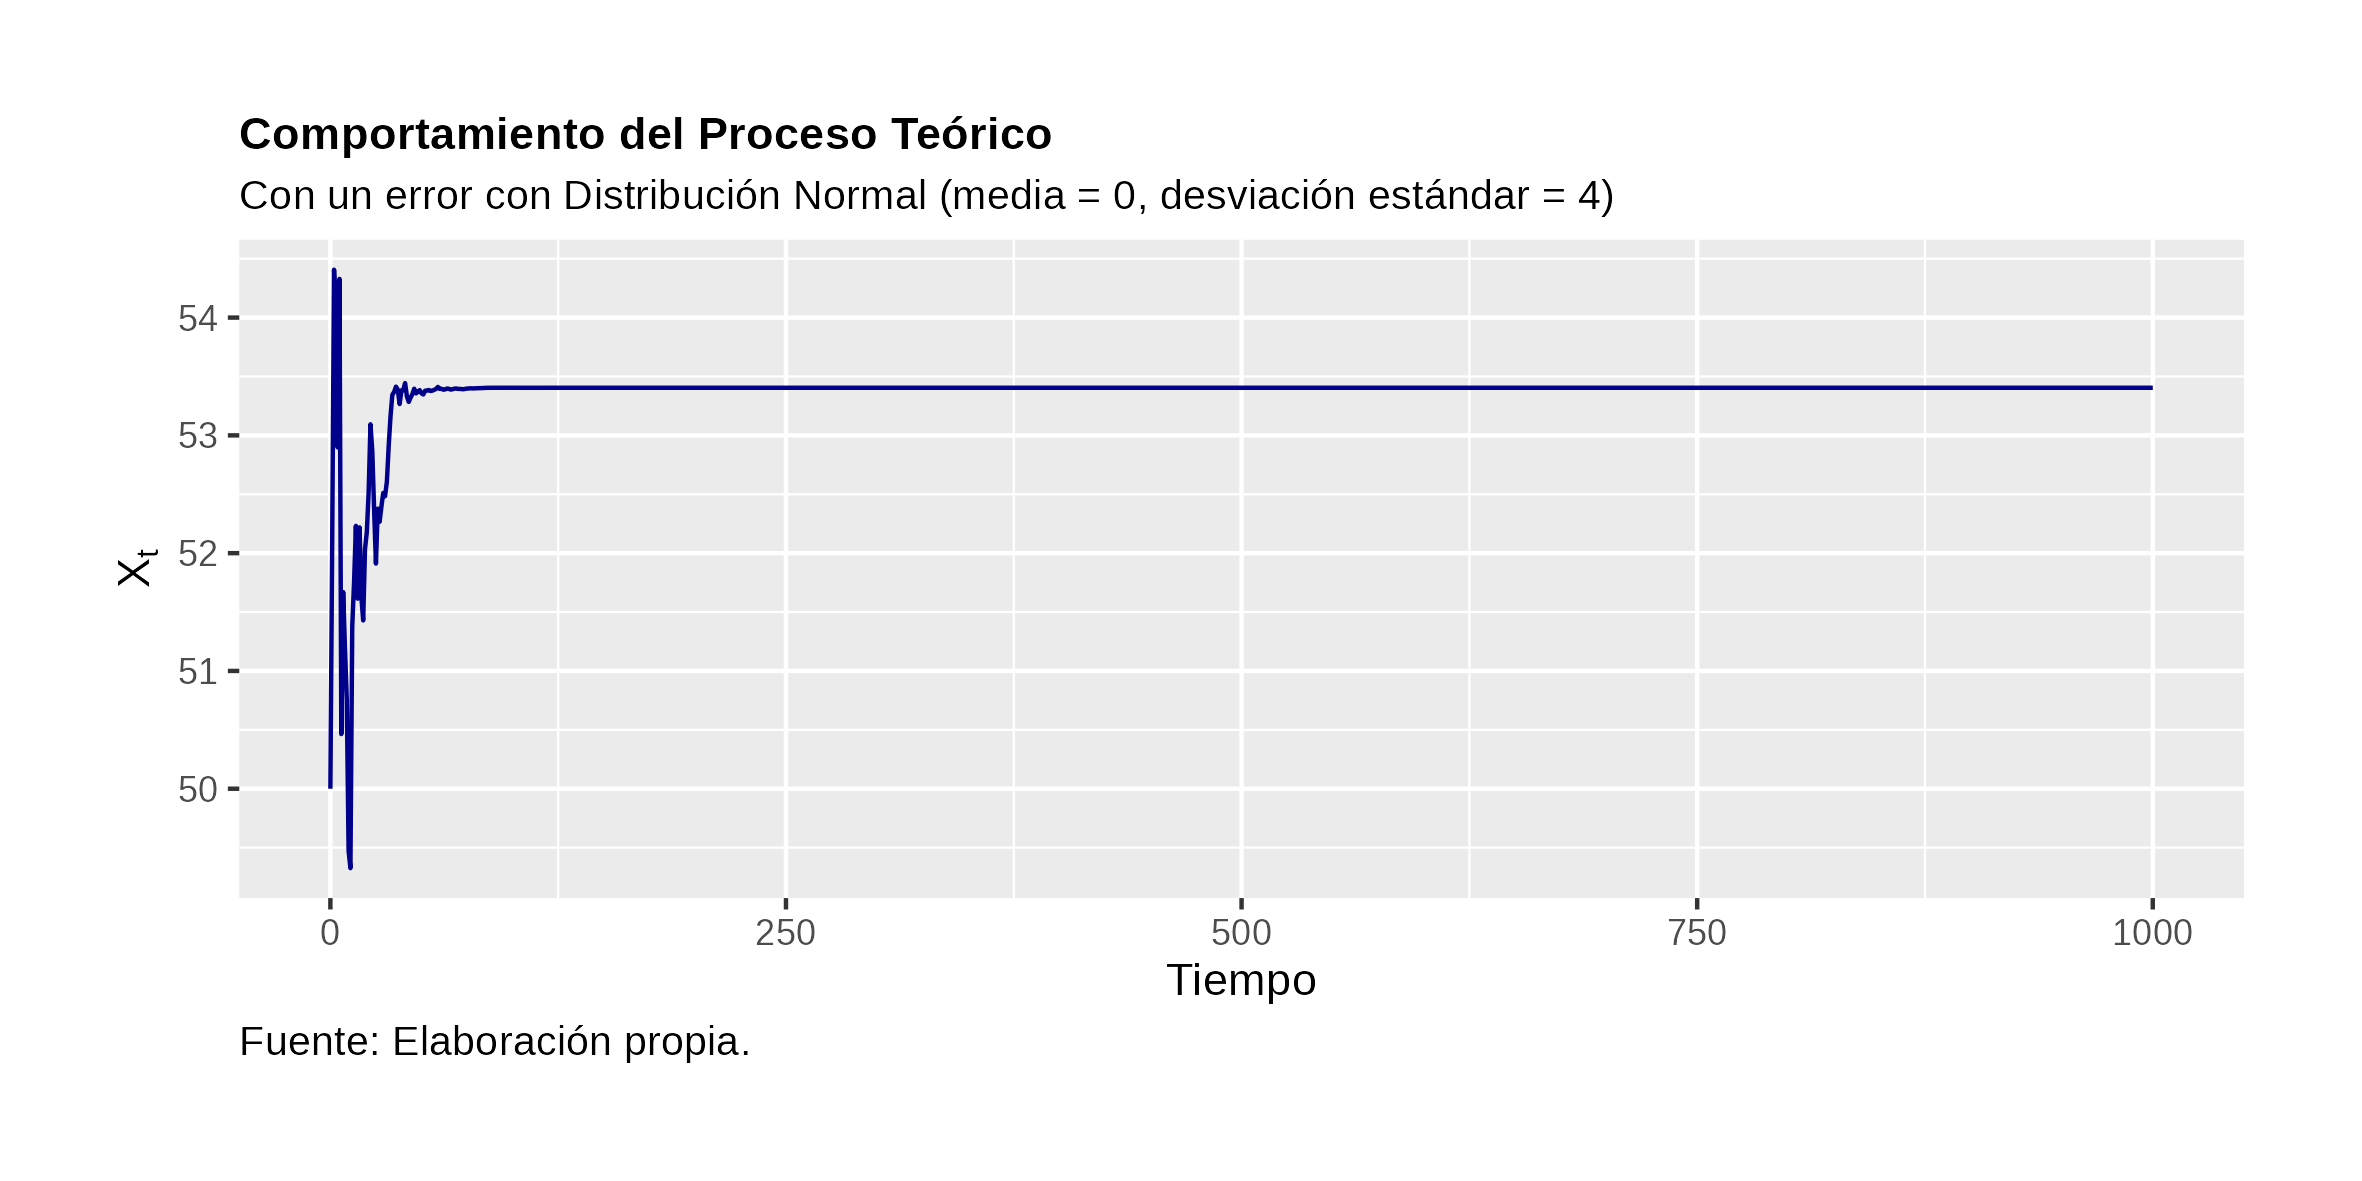
\includegraphics[width = 1.0 \textwidth]{G_AR_1_Teo}
  \caption{AR(1) considerando $X_t = \frac{5}{1 - 0.9} + \sum_{j = 0}^{t-1} 0.9^j U_{t-j}$, y que $U_t \sim \mathcal{N}(0, 4)$}
  \label{G_AR_1_Teo}
\end{figure}

\begin{figure}
  \centering
    \includegraphics[width=0.7 \textwidth]{G_AR_1_FACr}
  \caption{Función de autocorrelación de un AR(1): $\rho(\tau) = \frac{\gamma(\tau)}{\gamma(0)}$}
  \label{G_AR_1_FACr}
\end{figure}

\begin{figure}
  \centering
    \includegraphics[width=0.7 \textwidth]{G_AR_1_FACt}
  \caption{Función de autocorrelación de un AR(1): $\rho(\tau) = a_1^\tau$}
  \label{G_AR_1_FACt}
\end{figure}

Recordemos que una trayectoria de equilibrio o solución de un \(AR(1)\)
es como se muestra en la ecuación (\ref{AR1_Sol}). Así, nuestra serie
simulada cumple con la característica de que los errores son más
relevantes cuando la serie es corta. Por el contrario, los errores son
menos relevantes, cuando la serie es muy larga. La Figura
\ref{G_AR_1_Comb} ilustra esta observación de la trayectoria de
equilibrio.

\begin{figure}
  \centering
    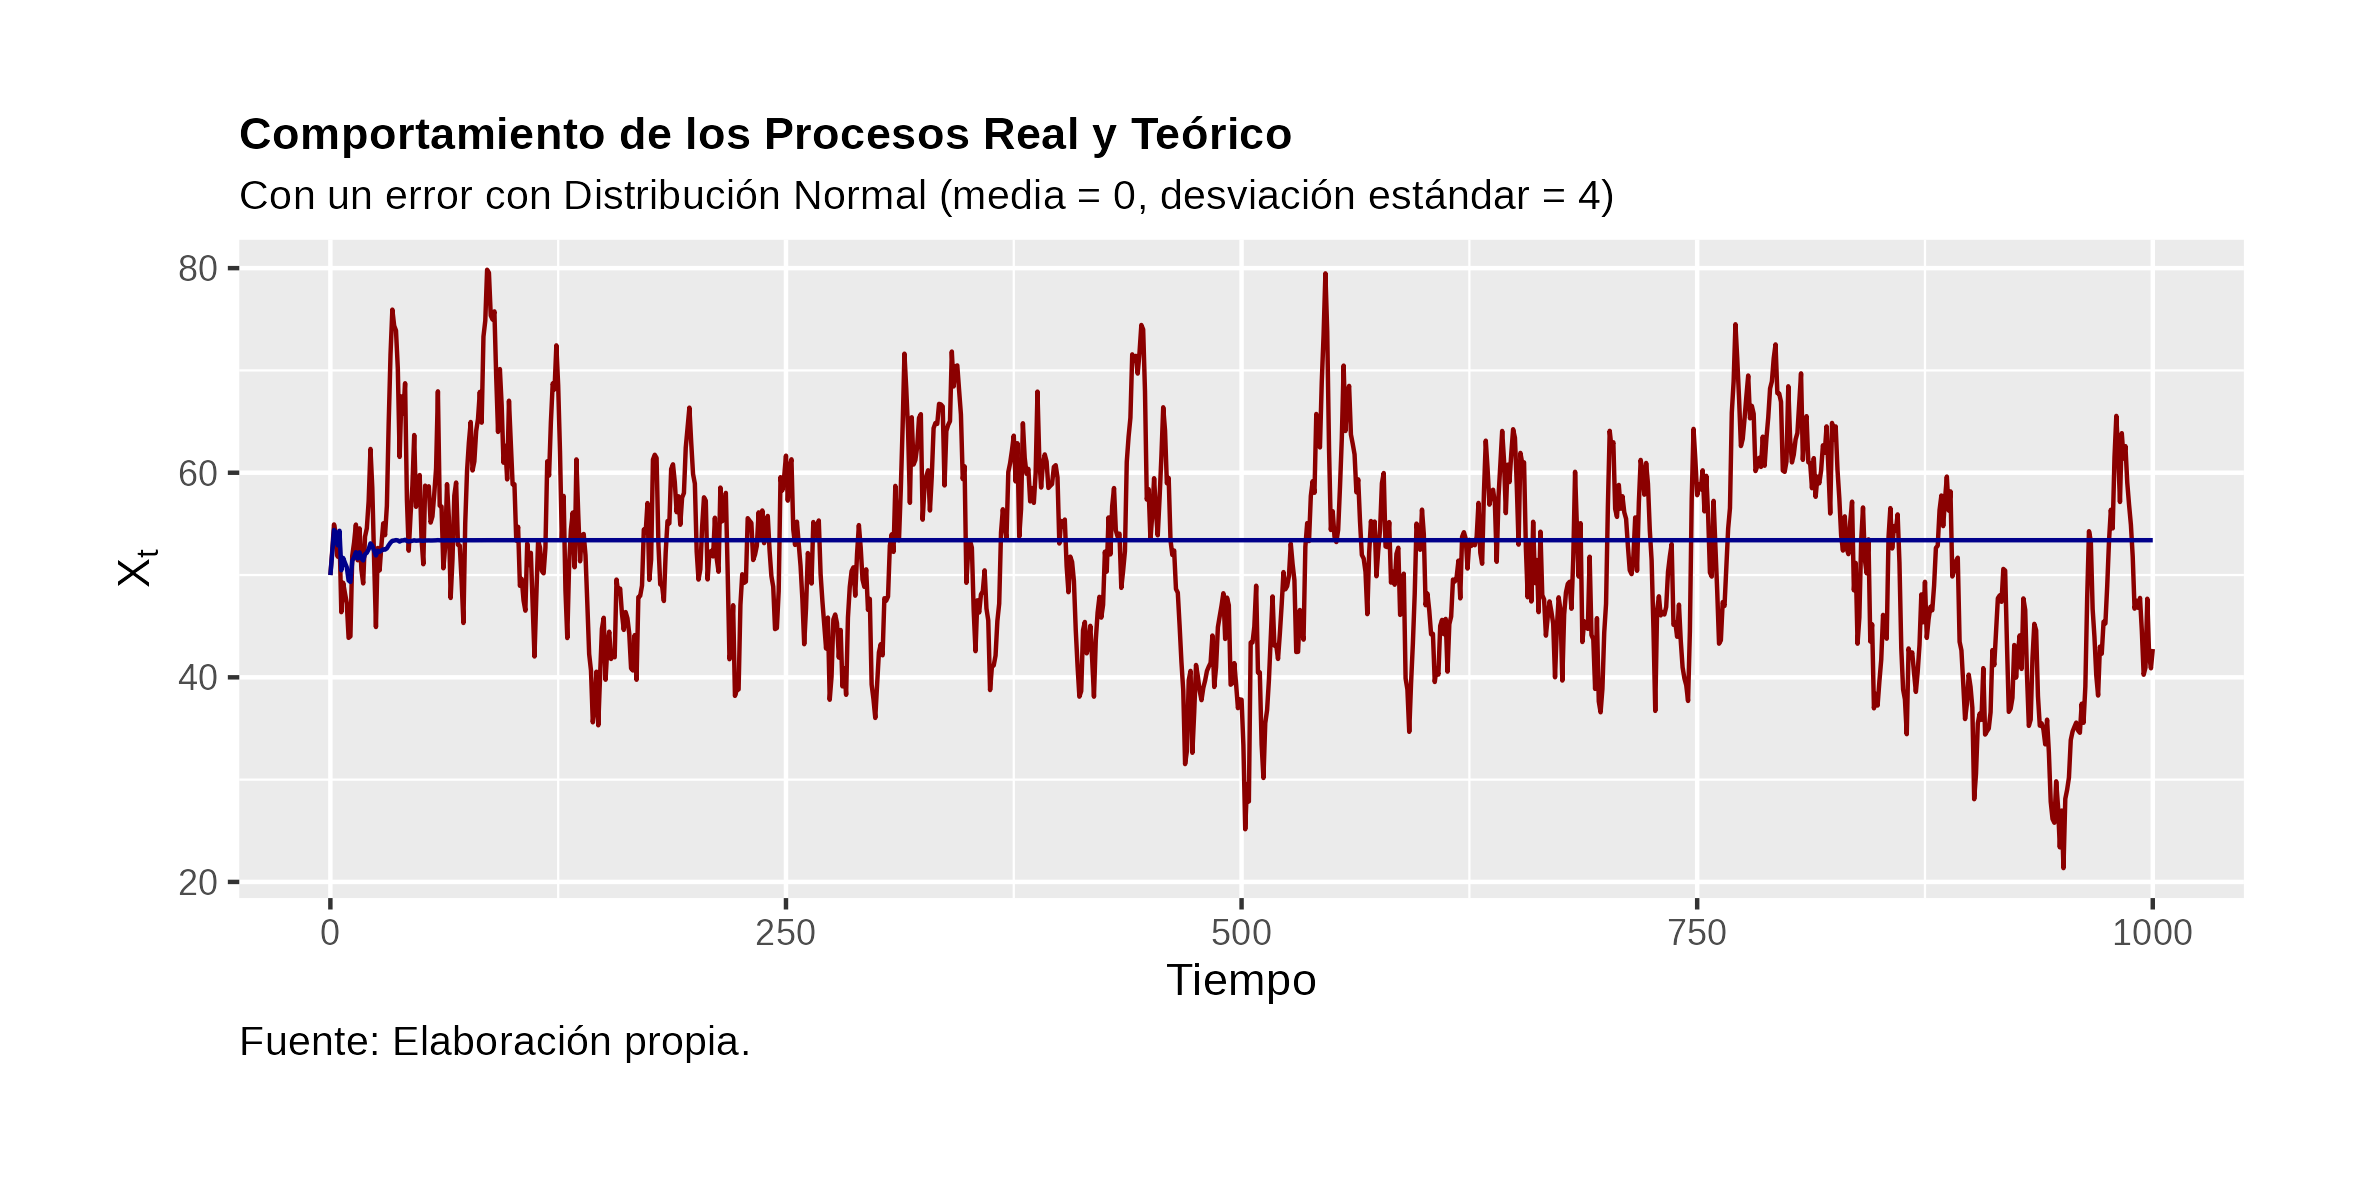
\includegraphics[width = 1.0 \textwidth]{G_AR_1_Comb}
  \caption{AR(1) considerando en conjunto $X_t = 5 + 0.9 X_{t-1} + U_t$; $X_0 = 50$ y $X_t = \frac{5}{1 - 0.9} + \sum_{j = 0}^{t-1} 0.9^j U_{t-j}$, y que $U_t \sim \mathcal{N}(0, 4)$}
  \label{G_AR_1_Comb}
\end{figure}

Para el segundo ejemplo consideremos una aplicación a una serie de
tiempo en especifico: Pasajeros transportados mensualmente en el Sistema
de Transporte Colectivo Metro (pasajeros medidos en
millones).\footnote{Fuente: INEGI, \url{https://www.inegi.org.mx/app/indicadores/?tm=0&t=1090}.}

A la serie se le aplicará una metodología de estimación dada por el
método de Máxima Verosimilitud (ML, por sus siglás en inglés). Antes de
realizar el proceso de estimación consideremos una transformación de
diferencias logaritmicas, con el objeto de obtener una serie de tiempo
expresada en tasas de
crecimiento\footnote{Estas no son porcentuales, para hacerlas porcentuales faltaría multiplicar por 100 a la serie.}
y con un comportamiento parecido a un proceso estacionario.

Así, para cada una de las series que analicemos en diferencias
logaritmicas las expresaremos bajo la siguiente transformación:

\[
    DLX_t = log(X_t) - log(X_{t-k})
\]

Donde \(k = 1, 2, 3, \ldots\) y \(log(.)\) es la función logaritmo
natural. Esta expresión se pude interpretar como una tasa de crecimiento
puesto que asumimos variaciones pequeñas para las cuales se cumple que:
\(log(X_t) - log(X_{t-k}) \approx \frac{X_t - X_{t-k}}{X_t}\).

Primero, al realizar el análisis de una serie de tiempo deberemos
decidir si éste se realizará para la serie en niveles o en diferencias.
Por convención, decimos que la series esta en niveles si ésta se analiza
sin heacerle ninguna transformación o si se analiza aplicando logarimos.
Cuando la serie se analiza en diferencias significa que la diferencia se
hace sin aplicar logaritmos o aplicando logaritmos. Sin embargo, lo
común es hacer un análisis en logaritmos.

Para decidir cómo analizar la serie de pasajeros en el metro de la CDMX
en la Figura \ref{G_Pax_Metro} se muestra la gráfica de la serie en
niveles (sin transformación logaritmica y con transformación
logarítmica) y en diferencias logarítmicas mensuales (es decir, con
\(k = 1\)).

\begin{figure}
  \centering
    \includegraphics[width = 1.0 \textwidth]{G_Pax_Metro}
  \caption{Pasajeros transportados (Millones) en el metro de la CDM en niveles y en diferencias logaritmicas.}
  \label{G_Pax_Metro}
\end{figure}

A continuación, estimaremos una \(AR(1)\) para la serie en niveles bajo
la transformación logaritmica (\(PaxLMetro_t\)) y en diferencias
logarítmitcas (\(PaxDLMetro_t\)). Para el primer caso obtenemos el
siguiente resultado:

\begin{center}
\begin{tabular}{ c c c c c c } 
    $PaxLMetro_t$ & $=$ & $4.8190$ & $+$ & $0.5916$  & $PaxLMetro_{t-1}$ \\ 
    &  & $(0.0105)$ &  & $(0.0526)$ & 
\end{tabular}
\end{center}

\begin{center}
\begin{tabular}{ c c c c c c c } 
    $\hat{\sigma}^2$ & $=$ & $0.004335$ & y & $AIC$ & $=$ & $-602.73$ 
\end{tabular}
\end{center}

Para el segundo caso obtenemos el siguiente resultado:

\begin{center}
\begin{tabular}{ c c c c c c } 
    $PaxDLMetro_t$ & $=$ & $0.0007$ & $-$ & $0.6194$  & $PaxDLMetro_{t-1}$ \\ 
    &  & $(0.0023)$ &  & $(0.0511)$ & 
\end{tabular}
\end{center}

\begin{center}
\begin{tabular}{ c c c c c c c } 
    $\hat{\sigma}^2$ & $=$ & $0.003344$ & y & AIC & $=$ & $-660.53$ 
\end{tabular}
\end{center}

En ambos casos observamos que el parámetro asociado al componente AR es
significativo y cumple con la restricción de ser en valor absoluto menor
a 1, por lo que la solución asociada al procesp será convergente.
También en ambos casos se reporta la estadística o Criterio de
Información de Akaike (AIC, por sus siglas en inglés), misma que más
adelante discutiremos su importancia y aplicación.

\hypertarget{ar2}{%
\subsubsection{AR(2)}\label{ar2}}

Una vez analizado el caso de \(AR(1)\) analizaremos el caso del
\(AR(2)\). La ecuación generalizada del proceso autoregresivo de orden 2
(denotado como \(AR(2)\)) puede ser escrito como:

\begin{equation}\protect\hypertarget{eq-AR2_Eq}{}{
X_t = a_0 + a_1 X_{t-1} + a_2 X_{t-2} + U_t
}\label{eq-AR2_Eq}\end{equation}

Donde \(U_t\) denota un proceso puramente aleatorio con media cero
(\(0\)), varianza constante (\(\sigma^2\)) y autocovarianza cero
(\(Cov(U_t, U_s) = 0\), con \(t \neq s\)), y un parametro
\(a_2 \neq 0\). Así, utilizando el operador rezago podemos reescribir la
ecuación (\ref{AR2_Eq}) como:

\begin{eqnarray*}
    X_t - a_1 X_{t-1} - a_2 X_{t-2} & = & a_0 + U_t \\
    (1 - a_1 L^1 - a_2 L^2) X_t & = & a_0 + U_t
\end{eqnarray*}

Donde, vamos a denotar a \(\alpha (L) = (1 - a_1 L^1 - a_2 L^2)\), y lo
llamaremos como un polinomio que depende del operador rezago y que es
distinto de cero. De esta forma podemos reescribir a la ecuación
(\ref{AR2_Eq}) como:

\[
\alpha(L) X_t = a_0 + U_t
\]

Ahora, supongamos que existe el inverso multiplicativo del polinomio
\(\alpha(L)\), el cual será denotado como: \(\alpha^{-1}(L)\) y cumple
con que:

\[
\alpha^{-1}(L) \alpha(L) = 1    
\]

Así, podemos escribir la solución a la ecuación (\ref{AR2_Eq}) como:

\[
    X_t = \alpha^{-1}(L) \delta + \alpha^{-1}(L) U_t
\]

Si utilizamos el hecho que \(\alpha^{-1}(L)\) se puede descomponer a
través del procedimiento de Wold en un polinomio de forma similar el
caso de \(AR(1)\), tenemos que:

\[
\alpha^{-1}(L) = \psi_0 + \psi_1 L + \psi_2 L^2 + \ldots
\]

Por lo tanto, el inverso multiplicativo \(\alpha^{-1}(L)\) se puede ver
como: \begin{equation}\protect\hypertarget{eq-InvAlpha}{}{
1 = (1 - a_1 L^1 - a_2 L^2) (\psi_0 + \psi_1 L + \psi_2 L^2 + \ldots)
}\label{eq-InvAlpha}\end{equation}

Desarrollando la ecuación (\ref{InvAlpha}) tenemos la sigueinte
expresión:

\begin{center}
\begin{tabular}{ c c c c c c c c c c c } 
    $1$ & $=$ & $\psi_0$ & $+$ & $\psi_1 L$ & $+$ & $\psi_2 L^2$ & $+$ & $\psi_3 L^3$ & $+$ & $\ldots$ \\
    $ $ & $ $ & $ $ & $-$ & $a_1 \psi_0 L$ & $-$ & $a_1 \psi_1 L^2$ & $-$ & $a_1 \psi_2 L^3$ & $-$ & $\ldots$ \\
    $ $ & $ $ & $ $ & $ $ & $ $ & $-$ & $a_2 \psi_0 L^2 $ & $-$ & $a_2 \psi_1 L^3$ & $-$ & $\ldots$
\end{tabular}
\end{center}

Ahora, podemos agrupar todos los términos en función del exponente
asociado al operador rezago \(L\). La siguiente es una solución
partícular y es una de las múltiples que podrían existir que cumpla con
la ecuación (\ref{InvAlpha}). Sin embargo, para efectos del análisis
sólo necesitamos una de esas soluciones. Utilizaremos las siguientes
condiciones que deben cumplirse en una de las posibles soluciones:

\begin{center}
\begin{tabular}{ c c c c } 
    $L^0 :$ & $ $ & $\Rightarrow$ & $\psi_0 = 1$ \\
    $L :$ & $\psi_1 - a_1 \psi_0 = 0$ & $\Rightarrow$ & $\psi_1 = a_1$ \\
    $L^2 :$ & $\psi_2 - a_1 \psi_1 - a_2 \psi_0 = 0$ & $\Rightarrow$ & $\psi_2 = a^2_1 + a_2$ \\
    $L^3 :$ & $\psi_3 - a_1 \psi_2 - a_2 \psi_1 = 0$ & $\Rightarrow$ & $\psi_3 = a^3_1 + 2 a_1 a_2$ \\
    $\vdots$ & $\vdots$ & $\vdots$ & $\vdots$
\end{tabular}
\end{center}

De esta forma podemos observar que en el límite siempre obtendremos una
ecuación del tipo \(\psi_j - a_1 \psi_{j-1} - a_2 \psi_{j-2} = 0\)
asociada a cada uno de los casos en que exista un \(L^j\), donde
\(j \neq 0, 1\), y la cual siempre podremos resolver conociendo que las
condiciones iniciales son: \(\psi_0 = 1\) y \(\psi_1 = a_1\).

Así, de las relaciones antes mencionadas y considerando que
\(\alpha^{-1} (L)\) aplicada a una constante como \(a_0\), tendrá como
resultado otra constante. De esta forma podemos escribir que la solución
del proceso AR(2) en la ecuación (\ref{AR2_Eq}) será dada por una
expresión como sigue:

\begin{equation}\protect\hypertarget{eq-AR2_Eq_Sol}{}{
X_t = \frac{\delta}{1 - a_1 - a_2} + \sum^{\infty}_{j = 0} \psi_{t - j} U_{t - j}
}\label{eq-AR2_Eq_Sol}\end{equation}

Donde todos los parametros \(\psi_i\) está determinado por los parámtros
\(a_0\), \(a_1\) y \(a_2\). En particular, \(\psi_0 = 1\) y
\(\psi_1 = a_1\) como describimos anteriormente. Al igual que en el caso
del \(AR(1)\), en la ecuación (\ref{AR2_Eq_Sol}) las condiciones de
estabilidad estarán dadas por las soluciones del siguiente polinomio
característico:\footnote{Note que raíces son equivalentes al inversio de las del polinomio dado por $\lambda^2 a_2 - \lambda a_1 - 1 = 0$.}

\[
\lambda^2 - \lambda a_1 - a_2 = 0
\]

Así, la condición de estabilidad de la trayectoria es que
\(\abs{\lambda_i} < 1\), para \(i = 1, 2\). Es decir, es necesario que
cada una de las raíces sea, en valor absoluto, siempre menor que la
unidad. Estas son las condiciones de estabilidad para el proceso
\(AR(2)\).

Finalmente, al igual que en un \(AR(1)\), a continuación determinamos
los momentos de una serie que sigue un proceso \(AR(2)\). Iniciamos con
la determinación de la media de la serie:

\[
\mathbb{E}[X_t] = \mu = \frac{a_0}{1 - a_1 - a_2}
\]

Lo anterior es cierto puesto que \(\mathbb{E}[U_{t - i}] = 0\), para
todo \(i = 0, 1, 2, \ldots\). Para determinar la varianza utilizaremos
las siguientes relaciones basadas en el uso del valor esperado, varianza
y covarianza de la serie. Adicionalmente, para simplificar el trabajo
asumamos que \(a_0 = 0\), lo cual implica que \(\mu = 0\). Dicho lo
anterior, partamos de: \begin{eqnarray*}
    \mathbb{E}[X_t X_{t - \tau}] & = & \mathbb{E}[(a_1 X_{t-1} + a_2 X_{t-2} + U_t) X_{t - \tau}]\\
    & = & a_1 \mathbb{E}[X_{t - 1} X_{t - \tau}] + a_2 \mathbb{E}[X_{t - 2} X_{t - \tau}] + \mathbb{E}[U_{t} X_{t - \tau}]
\end{eqnarray*}

Donde \(\tau = 0, 1, 2, 3, \ldots\) y que
\(\mathbb{E}[U_{t} X_{t - \tau}] = 0\) para todo
\(\tau \neq 0\).\footnote{ Es fácil demostrar está afirmación, sólo requiere de desarrollar la expresión y utilizar el hecho de que $U_t$ es un proceso pueramente aleatorio, por lo que la covarianza es cero (0).}
Dicho esto, podemos derivar el valor del valor esperado para diferentes
valores de \(\tau\):

\begin{center}
\begin{tabular}{ c c c c } 
    $\tau = 0:$ & $\gamma(0)$ & $=$ & $\alpha_1 \gamma(1) + \alpha_2 \gamma(2) + \sigma^2$ \\
    $\tau = 1:$ & $\gamma(1)$ & $=$ & $\alpha_1 \gamma(0) + \alpha_2 \gamma(1)$ \\
    $\tau = 2:$ & $\gamma(2)$ & $=$ & $\alpha_1 \gamma(1) + \alpha_2 \gamma(0)$ \\
    \vdots & \vdots & \vdots & \vdots
\end{tabular}
\end{center}

Donde debe ser claro que
\(\mathbb{E}[(X_{t} - \mu)(X_{t - \tau} - \mu)] = \mathbb{E}[X_{t} X_{t - \tau}] = \gamma(\tau)\).
Así, en general cuando \(\tau \neq 0\):

\[
\gamma(\tau) = a_1 \gamma(\tau - 1) + a_2 \gamma(\tau - 2)
\]

Realizando la sustitución recursiva y solucionando el sistema respectivo
obtenemos que las varianza y covarianzas estaran determinadas por:

\[
Var[X_t] = \gamma(0) = \frac{1 - a_2}{(1 + a_2)[(1 - a_2)^2 - a^2_1]} \sigma^2
\]

\[
\gamma(1) = \frac{a_1}{(1 + a_2)[(1 - a_2)^2 - a^2_1]} \sigma^2
\]

\[
\gamma(2) = \frac{a^2_1 + a_2 - a^2_2}{(1 + a_2)[(1 - a_2)^2 - a^2_1]} \sigma^2
\]

Recordemos que las funciones de autocorrelación se obtienen de la
división de cada unas de las funciones de covarianza (\(\gamma(\tau)\))
por la varianza (\(\gamma(0)\)). Así, podemos construir la siguiente
expresión:

\[
\rho(\tau) - a_1 \rho(\tau - 1) - a_2 \rho(\tau - 2) = 0
\]

Ahora veámos un ejemplo. Utilizaremos la serie de Pasajeros en vuelos
nacionales (en vuelos de salidas) para estimar un \(AR(2)\) mediante el
método de máxima verosimilitud (ML, por sus siglas en inglés). Antes de
realizar el proceso de estimación consideremos una transformación de la
serie en logaritmos y una más en diferencias logarítmicas; lo anterior
con el objeto de obtener un conjunto de series de tiempo suavizada y
expresada en tasas de crecimiento, con un comportamiento parecido a un
proceso estacionario.

Así, para cada una de las series que analicemos en diferencias
logarítmicas las expresaremos bajo la siguiente transformación:

\[
    DLX_t = log(X_t) - log(X_{t-k})
\]

Donde \(k = 1, 2, 3, \ldots\) y \(log(.)\) es la función logaritmo
natural. Por convención, decimos que la serie está en niveles si ésta se
analiza sin heacerle ninguna transformación o se analiza en logarimos.
Cuando la serie se analiza en diferencias significa que la diferencia se
hace sin aplicar logaritmos. Y cuando la serie analizada está en
diferenncias logarítmicas también diremos que esta en diferencias. Sin
embargo, lo común es hacer un análisis en logaritmos y en difereencias
logarítmicas.

Primero, para decidir si se realizará un AR(2) para la serie en niveles
o en diferencias analizaremos su gráfica. La serie en niveles, en
niveles bajo una transformación logarítmica y en diferencias
logarítmicas mensuales de los pasajeros en vuelos nacionales se muestra
en la Figura \ref{G_Pax_Nal}.

\begin{figure}
  \centering
    \includegraphics[width = 1.0 \textwidth]{G_Pax_Nal}
  \caption{Pasajeros en vuelos de salidas nacionales en niveles y en diferencias logaritmicas.}
  \label{G_Pax_Nal}
\end{figure}

A continuación, estimaremos un \(AR(2)\) para la serie en niveles bajo
una transformación logarítmica (\(LPaxNal_t\)) y en diferencias
logarítmitcas (\(DLPax_Nal_t\)). Para el primer caso obtenemos el
siguiente resultado:

\begin{center}
\begin{tabular}{ c c c c c c } 
    $LPaxNal_t$ & $=$ & $14.6267$ & $+$ & $0.7637$  & $LPaxNal_{t-1}$ \\ 
    &  & $(0.1816)$ &  & $(0.0637)$ & \\
    &  &  & $+$ & $0.2025$ & $LPaxNal_{t-2}$ \\
    &  &  &  & $(0.0646)$ &
\end{tabular}
\end{center}

\begin{center}
\begin{tabular}{ c c c c c c c } 
    $\hat{\sigma}^2$ & $=$ & $0.01138$ & y & $AIC$ & $=$ & $-372.64$ 
\end{tabular}
\end{center}

Para el segundo caso obtenemos el siguiente resultado:

\begin{center}
\begin{tabular}{ c c c c c c } 
    $DLPaxNal_t$ & $=$ & $0.0050$ & $-$ & $0.3205$  & $DLPaxNal_{t-1}$ \\ 
    &  & $(0.0036)$ &  & $(0.0592)$ & \\
    &  &  & $-$ & $0.4242$ & $DLPaxNal_{t-2}$ \\
    &  &  &  & $(0.0591)$ &
\end{tabular}
\end{center}

\begin{center}
\begin{tabular}{ c c c c c c c } 
    $\hat{\sigma}^2$ & $=$ & $0.009378$ & y & $AIC$ & $=$ & $-418.3$ 
\end{tabular}
\end{center}

Para ambos casos entre parentésis indicamos los errores estándar y
reportamos el estadístico de Akaike, AIC. Finalmente, podemos determinar
si las soluciones serán convergentes, para ello en la Figura
\ref{G_Roots_AR2} mostramos las raíces asociadas a cada uno de los
polinomios. De la inspección visual podemos concluir que ambas propuesta
de AR(2) representan una solución convergente y estable.

\begin{figure}
  \centering
    \includegraphics[width = 1.0 \textwidth]{G_Roots_AR2}
  \caption{Inveso de las Raíces del polinomio característico.}
  \label{G_Roots_AR2}
\end{figure}

\hypertarget{arp}{%
\subsubsection{AR(p)}\label{arp}}

Veremos ahora una generalización de los procesos autoregresivos (AR).
Esta generalización es conocida como un proceso \(AR(p)\) y que puede
ser descrito por la siguiente ecuación en diferencia estocástica:

\begin{equation}\protect\hypertarget{eq-ARp_Eq}{}{
X_t = a_0 + a_1 X_{t-1} + a_2 X_{t-2} + a_3 X_{t-3} + \ldots + a_p X_{t-p} + U_t
}\label{eq-ARp_Eq}\end{equation}

Donde \(a_p \neq 0\), y \(U_t\) es un proceso puramente aleatorio con
media cero (0), varianza constante (\(\sigma^2\)) y covarianza cero (0).
Usando el operador rezago, \(L^k\), para \(k = 0, 1, 2, \ldots, p\),
obtenemos la siguiente expresión de la ecuación (\ref{ARp_Eq}):

\[
(1 - a_1 L - a_2 L^2 - a_3 L^3 - \ldots - a_p L^p) X_t = a_0 + U_t
\]

Definamos el polinomio \(\alpha(L)\) como:

\begin{equation}\protect\hypertarget{eq-Pol_A}{}{
\alpha(L) = 1 - a_1 L - a_2 L^2 - a_3 L^3 - \ldots - a_p L^p
}\label{eq-Pol_A}\end{equation}

De forma similar que en los procesos \(AR(1)\) y \(AR(2)\), las
condiciones de estabilidad del proceso \(AR(p)\) estarán dadas por la
solución de la ecuación característica:

\[
\lambda^p - a_1 \lambda^{p-1} - a_2 \lambda^{p-2} - a_3 \lambda^{p-3} - \ldots - a_p = 0
\]

Así, solo si el polinomio anterior tiene raíces cuyo valor absoluto sea
menor a uno (\(\abs{\lambda_i} < 1\)) y si
\(1 - a_1 L - a_2 L^2 - a_3 L^3 - \ldots - a_p L^p < 1\) podremos decir
que el proceso es convergente y estable. Lo anterior significa que la
ecuación (\ref{Pol_A}) puede expresarse en términos de la descomposición
de Wold o como la suma infinita de términos como:

\[
\frac{1}{1 - a_1 L  - a_2 L^2 - a_3 L^3  - \ldots - a_p L^p} = \psi_0 + \psi_1 L + \psi_2 L^2 + \psi_3 L^3 + \ldots
\]

Donde, por construcción de \(\alpha(L) \alpha^{-1}(L) = 1\) implica que
\(\psi_0 = 1\). De forma similar a los proceso AR(1) y AR(2), es posible
determinar el valor de los coefieentes \(\psi_j\) en términos de los
coefientes \(a_i\). Así, la solución del proceso \(AR(p)\) estará dada
por:

\begin{equation}\protect\hypertarget{eq-ARp_Eq_Sol}{}{
X_t = \frac{a_0}{1 - a_1  - a_2 - a_3  - \ldots - a_p} + \sum^{\infty}_{j = 0} \psi_j U_{t-j}
}\label{eq-ARp_Eq_Sol}\end{equation}

Considerando la solución de la ecuación (\ref{ARp_Eq}) expresada en la
ecuación (\ref{ARp_Eq_Sol}) podemos determinar los momentos del proceso
y que estarán dados por una media como:

\[
\mathbb{E}[X_t] = \mu = \frac{a_o}{1 - a_1  - a_2 - a_3  - \ldots - a_p}
\]

Lo anterior, considerado que \(\mathbb{E}[U_t] = 0\), para todo \(t\).
Para determinar la varianza del proceso, sin pérdida de generalidad,
podemos definir una ecuación:
\(\gamma(\tau) = \mathbb{E}[X_{t - \tau} X_t]\), la cual (omitiendo la
constante, ya que la correlación de una constante con cuaquier variable
aleatoria que depende del tiempo es cero (0)) puede ser escrita como:

\[
\gamma(\tau) = \mathbb{E}[(X_{t - \tau}) \cdot (a_1 X_{t-1} + a_2 X_{t-2} + a_3 X_{t-3} + \ldots + + a_p X_{t-p} + U_t)]
\]

Donde \(\tau = 0, 1, 2, \ldots, p\) y \(a_0 = 0\), lo que implica que
\(\mu = 0\). De lo anterior obtenemos el siguiente conjunto de
ecuaciones mediante sustituciones de los valores de \(\tau\):

\begin{eqnarray}
    \gamma(0) & = & a_1 \gamma(1) + a_2 \gamma(2) + \ldots + a_p \gamma(p) + \sigma^2 \nonumber \\
    \gamma(1) & = & a_1 \gamma(0) + a_2 \gamma(1) + \ldots + a_p \gamma(p-1) \nonumber \\
    \vdots \nonumber \\
    \gamma(p) & = & a_1 \gamma(p-1) + a_2 \gamma(p-2) + \ldots + a_p \gamma(0) \nonumber
\end{eqnarray}

De esta forma, es fácil observar que la ecuación general para \(p > 0\)
estará dada por:

\begin{equation}\protect\hypertarget{eq-Gamma_p}{}{
\gamma(p) - a_1 \gamma(\tau - 1) - a_2 \gamma(\tau - 2) - \ldots - a_p \gamma(\tau - p) = 0
}\label{eq-Gamma_p}\end{equation}

Dividiendo la ecuación (\ref{Gamma_p}) por \(\gamma(0)\), se obtiene la
siguiente ecuación:

\[
\rho(p) - a_1 \rho(\tau - 1) + a_2 \rho(\tau - 2) + \ldots + a_p \rho(\tau - p) = 0
\]

Así, podemos escribir el siguiente sistema de ecuaciones:

\begin{eqnarray}
    \rho(1) & = & a_1 + a_2 \rho(1) + a_3 \rho(2) + \ldots + a_p \rho(p-1) \nonumber \\
    \rho(2) & = & a_1 \rho(1) + a_2 + a_3 \rho(1) + \ldots + a_p \rho(p-2) \nonumber \\
    & \vdots & \nonumber \\
    \rho(p) & = & a_1 \rho(p-1) + a_2 \rho(p-2) + \ldots + a_p \nonumber
\end{eqnarray}

Lo anterior se puede expresar como un conjunto de vectores y matrices de
la siguiente forma:

\[
    \left[ 
    \begin{array}{c}
        \rho(1) \\
        \rho(2) \\
        \vdots \\
        \rho(p)
    \end{array} 
    \right]
    = 
    \left[ 
    \begin{array}{c c c c}
        1 & \rho(1) & \ldots & \rho(p - 1) \\
        \rho(1) & 1 & \ldots & \rho(p - 2) \\
        \rho(2) & \rho(1) & \ldots & \rho(p - 3) \\
        \vdots & \vdots & \ldots & \vdots \\
        \rho(p - 1) & \rho(p - 2) & \ldots & 1 \\
    \end{array} 
    \right]
    \left[ 
    \begin{array}{c}
        a_1 \\
        a_2 \\
        a_3 \\
        \vdots \\
        a_p \\
    \end{array} 
    \right]
\]

De lo anterior podemos escribir la siguiente ecuación que es una forma
alternativa para expresar los valores de los coefientes \(a_i\) de la la
solución del proceso \(AR(p)\):

\[
\mathbf{\rho} = \mathbf{R} \mathbf{a}
\]

Es decir, podemos obtener la siguiente expresión:

\[
\mathbf{a} = \mathbf{R}^{-1} \mathbf{\rho}
\]

Ahora veámos un ejemplo. Utilizaremos la serie de Pasajeros en vuelos
internacionales de salida para estimar un \(AR(p)\) mediante el método
de máxima verosimilitud (ML). Antes de realizar el proceso de estimación
consideremos una transformación de la serie en logaritmos y una más en
diferencias logaritmicas; lo anterior con el objeto de obtener un
conjunto de series de tiempo suavizada y expresada en tasas de
crecimiento, con un comportamiento parecido a un proceso estacionario.

Primero, para decidir si se realizará un \(AR(p)\) para la serie en
niveles o en diferencias análizaremos su gráfica. La serie de e
Pasajeros en vuelos internacionales de salidas se muestra en la Figura
\ref{G_Pax_Int}. En está se muestra la gráfica de la serie en niveles
(sin transformación logaritmica y con transformación logaritmica) y en
diferencias logaritmicas mensuales (es decir, con diferencia respecto
del mes inmediato anterior).

\begin{figure}
  \centering
    \includegraphics[width = 1.0 \textwidth]{G_Pax_Int}
  \caption{Pasajeros en vuelos internacionales de salida en niveles y en diferencias logaritmicas.}
  \label{G_Pax_Int}
\end{figure}

De la gráfica en la Figura \ref{G_Pax_Int} observamos que quizá le mejor
forma de estimar un AR(p) es mediante la serie en diferencias, ya que
ésta es la que parece ser una serie estacionaria. A continuación,
estimaremos una AR(4) para la serie en diferencias logarimitcas
(\(DLPaxInt_t\)):

\begin{center}
\begin{tabular}{ c c c c c c } 
    $DLPaxInt_t$ & $=$ & $0.0050$ & $-$ & $0.2701$  & $DLPaxInt_{t-1}$ \\ 
    &  & $(0.0052)$ &  & $(0.0655)$ & \\
    &  &  & $-$ & $0.4326$ & $DLPaxNal_{t-2}$ \\
    &  &  &  & $(0.0664)$ & \\
    &  &  & $-$ & $0.1956$ & $DLPaxNal_{t-3}$ \\
    &  &  &  & $(0.0664)$ & \\
    &  &  & $-$ & $0.0316$ & $DLPaxNal_{t-4}$ \\
    &  &  &  & $(0.0653)$ & 
\end{tabular}
\end{center}

\begin{center}
\begin{tabular}{ c c c c c c c } 
    $\hat{\sigma}^2$ & $=$ & $0.02371$ & y & $AIC$ & $=$ & $-198.16$ 
\end{tabular}
\end{center}

Entre parentésis indicamos los errores estándar y reportamos el
estadístico de Akaike, AIC. Finalmente, podemos determinar si las
soluciones serán convergentes, para ello en la Figura \ref{G_Roots_ARp}
mostramos las raíces asociadas a cada uno de los polinomios. De la
inspección visual podemos concluir que el AR(4) representan una solución
convergente y estable.

\begin{figure}
  \centering
    \includegraphics[width = 0.7 \textwidth]{G_Roots_ARp}
  \caption{Inveso de las Raíces del polinomio característico.}
  \label{G_Roots_ARp}
\end{figure}

\hypertarget{procesos-de-medias-muxf3viles-ma}{%
\subsection{Procesos de Medias Móviles
(MA)}\label{procesos-de-medias-muxf3viles-ma}}

\hypertarget{ma1}{%
\subsubsection{MA(1)}\label{ma1}}

Una vez planteado el proceso generalizado de \(AR(p)\), iniciamos el
planteamiento de los proceso de medias móviles, denotados como
\(MA(q)\). Iniciemos con el planteamiento del proceso \(MA(1)\), que se
puede escribir como una ecuación como la siguiente:

\begin{equation}\protect\hypertarget{eq-MA1_Eq}{}{
X_t = \mu + U_t - b_1 U_{t-1}
}\label{eq-MA1_Eq}\end{equation}

O como:

\[
X_t - \mu = (1 - b_1 L) U_{t}
\]

Donde \(U_t\) es un proceso puramente aleatorio, es decir, con
\(\mathbb{E}[U_t] = 0\), \(Var[U_t] = \sigma^2\), y
\(Cov[U_t, U_s] = 0\). Así, un proceso \(MA(1)\) puede verse como un
proceso AR con una descomposición de Wold en la que \(\psi_0 = 1\),
\(\psi_1 = - b_1\) y \(\psi_j = 0\) para todo \(j > 1\).

Al igual que los procesos autoregresivos, determinaremos los momentos de
un proceso \(MA(1)\). En el caso de la media observamos que será:

\begin{eqnarray}
    \mathbb{E}[X_t] & = & \mu + \mathbb{E}[U_t] - b_1 \mathbb{E}[U_{t - 1}] \nonumber \\
    & = & \mu
\end{eqnarray}

Por su parte la varianza estará dada por: \begin{eqnarray}
    Var[X_t] & = & \mathbb{E}[(X_t - \mu)^2] \nonumber \\
    & = & \mathbb{E}[(U_t - b_1 U_{t-1})^2] \nonumber \\
    & = & \mathbb{E}[U_t^2 - 2 b_1 U_t U_{t-1} + b_1^2 U_{t - 1}^2] \nonumber \\
    & = &\mathbb{E}[U_t^2] - 2 b_1 \mathbb{E}[U_t U_{t-1}] + b_1^2 \mathbb{E}[U_{t - 1}^2]] \nonumber \\
    & = & \sigma^2 + b_1^2 \sigma^2 \nonumber \\
    & = & (1 + b_1^2) \sigma^2 = \gamma(0)
\end{eqnarray}

De esta forma, la varianza del proceso es constante en cualquier periodo
\(t\). Para determinar la covarianza utilizaremos la siguiente ecuación:

\begin{eqnarray}
    \mathbb{E}[(x_t - \mu)(x_{t + \tau} - \mu)] & = & \mathbb{E}[(U_t - b_1 U_{t-1})(U_{t + \tau} - b_1 U_{t + \tau - 1})] \nonumber \\
    & = & \mathbb{E}[U_t U_{t + \tau} - b_1 U_t U_{t + \tau - 1} - b_1 U_{t - 1} U_{t + \tau} \nonumber \\
    &   & + b_1^2 U_{t - 1} U_{t + \tau - 1}] \nonumber \\
    & = & \mathbb{E}[U_t U_{t + \tau}] - b_1 \mathbb{E}[U_t U_{t + \tau - 1}] \nonumber \\
    &   & - b_1 \mathbb{E}[U_{t - 1} U_{t + \tau}] + b_1^2 \mathbb{E}[U_{t - 1} U_{t + \tau - 1}]
    {#eq-MA1_Cov}
\end{eqnarray}

Si hacemos sustituciones de diferentes valores de \(\tau\) en la
ecuación (\ref{MA1_Cov}) notaremos que la covarianza será distinta de
cero únicamente para el caso de \(\tau = 1, -1\). En ambos casos
tendremos como resultado:

\begin{eqnarray}
    \mathbb{E}[(x_t - \mu)(x_{t + 1} - \mu)] & = & \mathbb{E}[(x_t - \mu)(x_{t - 1} - \mu)] \nonumber \\
    & = & - b_1 \mathbb{E}[U_t U_{t}] \nonumber \\
    & = & - b_1 \mathbb{E}[U_{t - 1} U_{t - 1}] \nonumber \\ 
    & = & - b_1^2 \sigma^2 = \gamma(1)
\end{eqnarray}

De esta forma tendremos que las funciones de autocorrelación estarán
dadas por los siguientes casos:

\begin{eqnarray}
    \rho(0) & = & 1 \nonumber \\
    \rho(1) & = & \frac{- b_1}{1 + b_1^2} \nonumber \\
    \rho(\tau) & = & 0 \text{ para todo } \tau > 1 \nonumber 
\end{eqnarray}

Ahora regresando a la ecuación (\ref{MA1_Eq}), su solución la podemos
expresar como:

\begin{eqnarray}
    U_ t & = & - \frac{\mu}{1 - b_1} + \frac{1}{1 - b_1 L} X_t \nonumber \\
    & = & - \frac{\mu}{1 - b_1} + X_t + b_1 X_{t-1} + b_1^2 X_{t-2} + \ldots \nonumber
\end{eqnarray}

Donde la condición para que se cumpla esta ecuación es que
\(\abs{b_1} < 1\). La manera de interpretar esta condición es como una
condición de estabilidad de la solución y cómo una condición de
invertibilidad. Notemos que un \(MA(1)\) (y en general un \(MA(q)\)) es
equivalente a un \(AR(\infty)\), es decir, cuando se invierte un MA se
genera un AR con infinitos rezagos.

En esta sección no desarrollaremos un ejemplo, primero explicaremos en
qué consiste una modelación del tipo \(MA(q)\) y después platearemos un
ejemplo en concreto.

\hypertarget{maq}{%
\subsubsection{MA(q)}\label{maq}}

En general, el proceso de medias móviles de orden \(q\), \(MA(q)\),
puede ser escrito como:

\begin{equation}\protect\hypertarget{eq-MAq_EQ}{}{
X_t = \mu + U_t - b_1 U_{t-1} - b_2 U_{t-2} - \ldots - b_q U_{t-q}
}\label{eq-MAq_EQ}\end{equation}

Podemos reescribir la ecuación (\ref{MAq_EQ}) utilizando el operador
rezago, así tendrémos el proceso de \(MA(q)\) como:

\begin{eqnarray}
    X_t - \mu & = & (1 - b_1 L - b_2 L^2 - \ldots - b_q L^q) U_{t} \nonumber \\
    X_t - \mu & = & \beta(L) U_t
\end{eqnarray} \{\#eq-MAq\_Red\}

Donde \(U_t\) es un proceso puramente aleatorio con
\(\mathbb{E}[U_t] = 0\), \(Var[U_t] = \mathbb{E}[U_t^2] = 0\) y
\(Cov[U_t, U_s] = \mathbb{E}[U_t, U_s] = 0\), y
\(\beta(L) = 1 - b_1 L - b_2 L^2 - \ldots - b_q L^q\) es un polinomio
del operador rezago \(L\). la ecuación (\ref{MAq_Red}) puede ser
interpretada como un proceso \(AR(q)\) sobre la serie \(U_t\).

Ahora determinemos los momentos de un proceso \(MA(q)\):

\begin{eqnarray}
    \mathbb{E}[X_t] & = & \mathbb{E}[\mu + U_t - b_1 U_{t-1} - b_2 U_{t-2} - \ldots - b_q U_{t-q}] \nonumber \\
    & = & \mu + \mathbb{E}[U_t] - b_1 \mathbb{E}[U_{t-1}] - b_2 \mathbb{E}[U_{t-2}] - \ldots - b_q \mathbb{E}[U_{t-q}] \nonumber \\
    & = & \mu
\end{eqnarray}

En el caso de la varianza tenemos que se puede expresar como:

\begin{eqnarray}
    Var[X_t] & = & \mathbb{E}[(X_t - \mu)^2] \nonumber \\
    & = & \mathbb{E}[(U_t - b_1 U_{t-1} - b_2 U_{t-2} - \ldots - b_q U_{t-q})^2] \nonumber \\
    & = & \mathbb{E}[U_t^2 + b_1^2 U_{t-1}^2 + b_2^2 U_{t-2}^2 + \ldots + b_q^2 U_{t-q}^2 \nonumber \\
    &   & - 2 b_1 U_t U_{t - 1} - \ldots - 2 b_{q - 1} b_q U_{t - q + 1} U_{t - q}] \nonumber \\
    & = & \mathbb{E}[U_t^2] + b_1^2 \mathbb{E}[U_{t-1}^2] + b_2^2 \mathbb{E}[U_{t-2}^2] + \ldots + b_q^2 \mathbb{E}[U_{t-q}^2] \nonumber \\
    &   & - 2 b_1 \mathbb{E}[U_t U_{t - 1}] - \ldots - 2 b_{q - 1} b_q \mathbb{E}[U_{t - q + 1} U_{t - q}] \nonumber \\
    & = & \sigma^2 + b^2_1 \sigma^2 + b^2_2 \sigma^2 + \ldots + b^2_q \sigma^2 \nonumber \\
    & = & (1 + b^2_1 + b^2_2 + \ldots + b^2_q) \sigma^2
\end{eqnarray}

En el caso de las covarianzas podemos utilizar una idea similar al caso
del \(AR(p)\), construir una expresión general para cualquier rezago
\(\tau\):

\begin{eqnarray}
    Cov[X_t, X_{t + \tau}] & = & \mathbb{E}[(X_t - \mu)(X_{t + \tau} - \mu)] \nonumber \\
    & = & \mathbb{E}[(U_t - b_1 U_{t-1} - b_2 U_{t-2} - \ldots - b_q U_{t-q}) \nonumber \\
    &   & (U_{t + \tau} - b_1 U_{t + \tau -1} - b_2 U_{t + \tau -2} - \ldots - b_q U_{t + \tau - q})] \nonumber
\end{eqnarray}

La expresión anterior se puede desarrollar para múltiples casos de
\(\tau = 1, 2, \ldots, q\). De esta forma tenemos el siguiente sistema:

\begin{eqnarray}
    \tau = 1 & : & \gamma(1) = (- b_1 + b_1 b_2 + \ldots + b_{q-1} b_q) \sigma^2 \nonumber \\
    \tau = 2 & : & \gamma(2) = (- b_2 + b_1 b_3 + \ldots + b_{q-2} b_q) \sigma^2 \nonumber \\
    & \vdots & \nonumber \\
    \tau = q & : & \gamma(q) = b_q \sigma^2 \nonumber
\end{eqnarray}

Donde \(\gamma(\tau) = 0\) para todo \(\tau > q\). Es decir, todas las
autocovarianzas y autocorrelaciones con ordenes superiores a \(q\) son
cero (0). De esta forma, esta caracterítica teórica permite identificar
el orden de \(MA(q)\) visualizando la función de autocorrelación y
verificando a partir de cual valor de rezago la autocorrelación es no
significaiva.

Regresando al problema original que es el de determinar una solución
para la eucación (\ref{MAq_EQ}), tenemos que dicha solución estará dada
por un \(AR(\infty)\) en términos de \(U_t\):

\begin{eqnarray}
    U_t & = & - \frac{\mu}{1 - b_1 - b_2 - \ldots - b_q} + \beta(L)^{-1} X_t \nonumber \\
    &   & - \frac{\mu}{1 - b_1 - b_2 - \ldots - b_q} + \sum_{j = 0}^{\infty} c_j X_{t-j} 
\end{eqnarray} \{\#eq-MAq\_Eq\_Sol\}

Donde se cumple que:
\(1 = (1 - b_1 L^1 - b_2 L^2 - \ldots - b_q L^q)(1 - c_1 L - c_2 L^2 - \ldots)\)
y los coeficientes \(c_j\) se pueden determinar por un método de
coeficientes indeterminados y en términos de los valores \(b_i\). De
igual forma que en el caso de la ecuación (\ref{ARp_Eq}), en la ecuación
(\ref{MAq_Eq_Sol}) se deben cumplir condiciones de estabilidad asociadas
con las raíces del polinomio carácterististico dado por:

\[
1 - b_1 x - b_2 x^2 - \ldots b_q x^q = 0
\]

El cual debe cumplir que \(\abs{x_i} < 1\) y que
\(1 - b_1 - b_2 - \ldots b_q < 1\).

Ahora veamos un ejemplo del proceso \(MA(q)\), para lo cual retomaremos
la serie de Pasajeros transportados en el metro de la CDMX
(\(PaxMetro\)). Estimaremos el \(MA(q)\) mediante el método de máxima
verosimilitud (ML). Antes de realizar el proceso de estimación
consideremos una transformación de la serie en logaritmos y una más en
diferencias logaritmicas; lo anterior con el objeto de obtener un
conjunto de series de tiempo suavizada y expresada en tasas de
crecimiento, con un comportamiento parecido a un proceso estacionario.

La serie de Pasajeros transportados en el metro de la CDMX se muestra en
la Figura \ref{G_Pax_Metro} se muestra la gráfica de la serie en niveles
(sin transformación logarítmica y con transformación logarítmica) y en
diferencias logarítmicas mensuales (es decir, con una diferencia
respecto del mes inmediato anterior). Utilizaremos la serie en
diferencias, ya que es la que parece ser estacionaria. Esta serie tiene
la peculiaridad de que tiene un salto a la baja y uno al alza entre
septiembre de 2017 y octubre de 2017. Para controlar ese efecto, en
nuestro modelo \(MA(q)\) incluiremos dos variables dummies para dichos
meses.

A continuación, estimaremos una \(MA(4)\) para la serie en diferencias:

\begin{center}
\begin{tabular}{ c c c c c c } 
    $DLPaxMetro_t$ & $=$ & $0.0000$ & $-$ & $0.7804$  & $U_{t-1}$ \\ 
    &  & $(0.0000)$ &  & $(0.0661)$ & \\
    &  &  & $+$ & $0.3591$ & $U_{t-2}$ \\
    &  &  &  & $(0.0826)$ & \\
    &  &  & $-$ & $0.2775$ & $U_{t-3}$ \\
    &  &  &  & $(0.0908)$ & \\
    &  &  & $-$ & $0.1120$ & $U_{t-4}$ \\
    &  &  &  & $(0.0769)$ & \\
    &  &  & $-$ & $0.3789$ & $DSep2017$ \\
    &  &  &  & $(0.0436)$ & \\
    &  &  & $+$ & $0.3695$ & $DOct2017$ \\
    &  &  &  & $(0.0434)$ & 
\end{tabular}
\end{center}

\begin{center}
\begin{tabular}{ c c c c c c c } 
    $\hat{\sigma}^2$ & $=$ & $0.002176$ & y & $AIC$ & $=$ & $-749.94$ 
\end{tabular}
\end{center}

Entre parentésis indicamos los errores estándar y al final reportamos el
estadístico de Akaike, AIC. Finalmente, podemos determinar si la
solución serán convergente, para ello en la Figura \ref{G_Roots_MAq}
mostramos las raíces asociadas a cada uno de los polinomios. De la
inspección visual podemos concluir que ambas propuesta de AR(2)
representan una solución convergente y estable.

\begin{figure}
  \centering
    \includegraphics[width = 1.0 \textwidth]{G_Roots_MAq}
  \caption{Inveso de las Raíces del polinomio característico.}
  \label{G_Roots_MAq}
\end{figure}

\hypertarget{procesos-armap-q-y-arimap-d-q}{%
\subsection{Procesos ARMA(p, q) y ARIMA(p, d,
q)}\label{procesos-armap-q-y-arimap-d-q}}

Hemos establecido algunas relaciones las de los porcesos AR y los
procesos MA, es decir, cómo un \(MA(q)\) de la serie \(X_t\) puede ser
reexpresada como un \(AR(\infty)\) de la serie \(U_t\), y viceversa un
\(AR(p)\) de la serie \(X_t\) puede ser reeexpresada como un
\(MA(\infty)\).

En este sentido, para cerrar esta sección veámos el caso de la
especificación que conjunta ambos modelos en un modelo general conocido
como \(ARMA(p, q)\) o \(ARIMA(p, d, q)\). La diferencia entre el primero
y el segundo es las veces que su tuvo que diferenciar la serie
analizada, registro que se lleva en el índice \(d\) de los paramétros
dentro del concepto \(ARIMA(p, d, q)\). No obstante, en general nos
referiremos al modelo como \(ARMA(p, q)\) y dependerá del analista si
modela la serie en niveles (por ejemplo, en logaritmos) o en diferencias
logarítmicas (o diferencias sin logaritmos).

\hypertarget{arma1-1}{%
\subsubsection{ARMA(1, 1)}\label{arma1-1}}

Dicho lo anterior vamos a empezar con el análisis de un \(ARMA(1, 1)\).
Un proceso \(ARMA(1, 1)\) puede verse como:

\begin{equation}\protect\hypertarget{eq-ARMA11_Eq}{}{
X_t = \delta + a_1 X_{t - 1} + U_t - b_1 U_{t - 1}
}\label{eq-ARMA11_Eq}\end{equation}

Aplicando el operado rezago podemos rescribir la ecuación
(\ref{ARMA11_Eq}) como: \[
(1 - a_1 L) X_t = \delta + (1 - b_1 L) U_t
\]

Donde \(U_t\) es un proceso pueramente aleatorio como en los casos de
\(AR(p)\) y \(MA(q)\), y \(X_t\) puede ser una serie en niveles o en
diferencias (ambas, en términos logarítmicos).

Así, el modelo \(ARIMA (p, q)\) también tiene una representación de Wold
que estará dada por las siguientes expresiones:

\begin{equation}\protect\hypertarget{eq-ARMA11_Prev}{}{
X_t = \frac{\delta}{1 - a_1} + \frac{1 - b_1 L}{1 - a_1 L} U_t
}\label{eq-ARMA11_Prev}\end{equation}

Donde \(a_1 \neq b_1\), puesto que en caso contrario \(X_t\) sería un
proceso puramente aleatorio con una media
\(\mu = \frac{\delta}{1 - a_1}\). Así, podemos reescribir la
descomposición de Wold a partir del componente de la ecuación
(\ref{ARMA11_Prev}):

\begin{equation}\protect\hypertarget{eq-ARMA11_EQ_Wold}{}{
\frac{1 - b_1 L}{1 - a_1 L} = \psi_0 + \psi_1 L + \psi_2 L^2 + \psi_3 L^3 + \ldots 
}\label{eq-ARMA11_EQ_Wold}\end{equation}

Está ecuación es equivalente a la expresión:

\begin{eqnarray}
    (1 - b_1 L) & = & (1 - a_1 L)(\psi_0 + \psi_1 L + \psi_2 L^2 + \psi_3 L^3 + \ldots) \nonumber \\
    & = & \psi_0 + \psi_1 L + \psi_2 L^2 + \psi_3 L^3 + \ldots \nonumber \\
    &   & - a_1 \psi_0 L - a_1 \psi_1 L^2 - a_2 \psi_2 L^3 - a_1 \psi_3 L^4 - \ldots \nonumber
\end{eqnarray}

De esta forma podemos establecer el siguiente sistema de coeficientes
indeterminados:

\begin{center}
\begin{tabular}{ c c c c } 
    $L^0 :$ & $ $ & $\Rightarrow$ & $\psi_0 = 1$ \\
    $L^1 :$ & $\psi_1 - a_1 \psi_0 = - b_1$ & $\Rightarrow$ & $\psi_1 = a_1 - b_1$ \\
    $L^2 :$ & $\psi_2 - a_1 \psi_1 = 0$ & $\Rightarrow$ & $\psi_2 = a_1(a_1 - b_1)$ \\
    $L^3 :$ & $\psi_3 - a_1 \psi_2 = 0$ & $\Rightarrow$ & $\psi_3 = a^2_1(a_1 - b_1)$ \\
    $\vdots$ & $\vdots$ & $\vdots$ & $\vdots$ \\
    $L^j :$ & $\psi_j - a_1 \psi_{j - 1} = 0$ & $\Rightarrow$ & $\psi_j = a^{j - 1}_1(a_1 - b_1)$
\end{tabular}
\end{center}

Así, la solución a la ecuación (\ref{ARMA11_Eq}) estará dada por la
siguiente generalización:

\begin{equation}\protect\hypertarget{eq-ARMA11_Sol}{}{
X_t = \frac{\delta}{1 - a_1} + U_t + (a_1 - b_1) U_{t - 1} + a_1(a_1 - b_1) U_{t - 2} + a_1^2(a_1 - b_1) U_{t - 3} + \ldots
}\label{eq-ARMA11_Sol}\end{equation}

En la ecuación (\ref{ARMA11_Sol}) las condiciones de estabilidad y de
invertibilidad del sistema (de un MA a un AR, y viceversa) estarán dadas
por: \(\abs{a_1} < 1\) y \(\abs{b_1} < 1\). Adicionalmente, la ecuación
(\ref{ARMA11_Sol}) expresa cómo una serie que tiene un comportamiento
\(ARMA(1, 1)\) es equivalente a una serie modelada bajo un
\(MA(\infty)\).

Al igual que en los demás modelos, ahora determinaremos los momentos del
proceso \(ARMA(1, 1)\). La media estará dada por:

\begin{eqnarray}
    \mathbb{E}[X_t] & = & \mathbb{E}[\delta + a_1 X_{t-1} + U_t - b_1 U_{t-1}] \nonumber \\
    & = & \delta + a_1 \mathbb{E}[X_{t-1}] \nonumber \\
    & = & \frac{\delta}{1 - a_1} \nonumber \\
    & = & \mu
\end{eqnarray}

Donde hemos utilizado que
\(\mathbb{E}[X_t] = \mathbb{E}[X_{t-1}] = \mu\). Es decir, la media de
un \(ARMA(1, 1)\) es idéntica a la de un \(AR(1)\).

Para determinar la varianza tomaremos una estrategía similar a los casos
de \(AR(p)\) y \(MA(q)\). Por lo que para todo \(\tau \geq 0\), y
suponiendo por simplicidad que \(\delta = 0\) (lo que implica que
\(\mu = 0\)) tendremos:

\begin{eqnarray}
    \mathbb{E}[X_{t-\tau} X_t] & = & \mathbb{E}[(X_{t-\tau}) \cdot (a_1 X_{t-1} + U_t - b_1 U_{t-1})] \nonumber \\
    & = & a_1 \mathbb{E}[X_{t-\tau} X_{t-1}] + \mathbb{E}[X_{t-\tau} U_t] - b_1 \mathbb{E}[X_{t-\tau} U_{t-1}]
    {#eq-ARMA11_Cov}
\end{eqnarray}

De la ecuación (\ref{ARMA11_Cov}) podemos determinar una expresión para
el caso de \(\tau = 0\):

\begin{eqnarray}
    \mathbb{E}[X_{t} X_t] & = & \gamma(0) \nonumber \\
    & = & a_1 \gamma(1) + \mathbb{E}[U_t X_t] - b_1 \mathbb{E}[X_t U_{t-1}] \nonumber \\
    & = & a_1 \gamma(1) + \sigma^2 + b_1 \mathbb{E}[U_{t-1} (a_1 X_{t-1} + U_t - b_1 U_{t-1})] \nonumber \\
    & = & a_1 \gamma(1) + \sigma^2 - b_1 a_1 \sigma^2 + b_1 \sigma^2 \nonumber \\
    & = & a_1 \gamma(1) + (1 - b_1 (a_1 - b_1)) \sigma^2
\end{eqnarray}

Para el caso en que \(\tau = 1\):

\begin{eqnarray}
    \mathbb{E}[X_{t-1} X_t] & = & \gamma(1) \nonumber \\
    & = & a_1 \gamma(0) + \mathbb{E}[X_{t-1} U_t] - b_1 \mathbb{E}[X_{t-1} U_{t-1}] \nonumber \\
    & = & a_1 \gamma(0) - b_1 \sigma^2
\end{eqnarray}

Estas últimas expresiones podemos resolverlas como sistema para
determinar los siguientes valores:

\begin{eqnarray}
    \gamma(0) & = & \frac{1 + b_1^2 - 2 a_1 b_1}{1 - a_1^2} \sigma^2 \\
    \gamma(1) & = & \frac{(a_1 - b_1)(1 - a_1 b_1)}{1 - a_1^2} \sigma^2
\end{eqnarray}

En general para cualquier valor \(\tau \geq 2\) tenemos que la
autocovarianza y la función de autocorrelación serán:

\begin{eqnarray}
    \gamma(\tau) = a_1 \gamma(\tau - 1) \\
    \rho(\tau) = a_1 \rho(\tau - 1)
\end{eqnarray}

Por ejemplo, para el caso de \(\tau = 1\) tendríamos:

\[
\rho(1) = \frac{(a_1 - b_1)(1 - a_1 b_1)}{1 + b_1^2 - 2 a_1 b_1}
\]

De esta forma, la función de autocorrelación oscilará en razón de los
valores que tome \(a_1\) y \(b_1\).

\hypertarget{armap-q}{%
\subsubsection{ARMA(p, q)}\label{armap-q}}

La especificación general de un \(ARMA(p, q)\) (donde
\(p, q \in \mathbb{N}\)) puede ser descrita por la siguiente ecuación:

\begin{eqnarray}
    X_t & = & \delta + a_1 X_{t - 1} + a_2 X_{t - 2} + \ldots + a_p X_{t - p} \nonumber \\
    &   & + U_t - b_1 U_{t - 1} - b_2  U_{t - 2} - \ldots - b_q  U_{t - q}
\end{eqnarray} \{\#eq-ARMApq\_Eq\}

Donde \(U_t\) es un proceso puramente aleatorio, y \(X_t\) puede ser
modelada en niveles o en diferencias (ya sea en logaritmos o sin
transformación logarítmica).

Mediante el uso del operador rezago se puede escribir la ecuación
(\ref{ARMApq_Eq}) como:

\begin{equation}\protect\hypertarget{eq-ARMApq_EQLag}{}{
(1 - a_1 L - a_2 L^2 - \ldots - a_p L^p) X_t = \delta + (1 - b_1 L - b_2 L^2 - \ldots - b_q L^q) U_t 
}\label{eq-ARMApq_EQLag}\end{equation}

En la ecuación (\ref{ARMApq_EQLag}) definamos dos polinomios:
\(\alpha(L) = (1 - a_1 L - a_2 L^2 - \ldots - a_p L^p)\) y
\(\beta(L) = (1 - b_1 L - b_2 L^2 - \ldots - b_q L^q)\). Así, podemos
reescribir la ecuación (\ref{ARMApq_EQLag}) como:

\[
\alpha(L) X_t = \delta + \beta(L) U_t 
\]

Asumiendo que existe el polinomio inverso tal que:
\(\alpha(L)^{-1}\alpha(L) = 1\).La solución entonces puede ser escrita
como:

\begin{eqnarray}
    X_t & = & \alpha(L)^{-1} \delta + \alpha(L)^{-1} \beta(L) U_t \nonumber \\
    & = & \frac{\delta}{1 - a_1 - a_2 - \ldots - a_p} + \frac{\beta(L)}{\alpha(L)} U_t \nonumber \\
    & = & \frac{\delta}{1 - a_1 - a_2 - \ldots - a_p} + U_t + \psi_1 L U_t + \psi_2 L^2 U_t + \ldots
\end{eqnarray} \{\#eq-ARMApq\_Wold\}

Donde la ecuación (\ref{ARMApq_Wold}) nos permite interpretar que un
ARMA(p, q) se puede reexpresar e interpreetar como un \(MA(\infty)\) y
donde las condiciones para la estabilidad de la solución y la
invertibilidad es que las ráices de los polinomios característicos
\(\alpha(L)\) y \(\beta(L)\) son en valor absoluto menores a 1.

Adicionalmente, la fracción en la ecuación (\ref{ARMApq_Wold}) se puede
descomponer como en la forma de Wold:

\[
\frac{\beta(L)}{\alpha(L)} = 1 + \psi_1 L + \psi_2 L^2 + \ldots
\]

Bajo los supuestos de estacionariedad del componente \(U_t\), los
valores de la media y varianza de un proceso \(ARMA(p, q)\) serán como
describimos ahora. Para el caso de la media podemos partir de la
ecuación (\ref{ARMApq_Wold}) para generar:

\begin{eqnarray}
    \mathbb{E}[X_t] & = & \mathbb{E}\left[ \frac{\delta}{1 - a_1 - a_2 - \ldots - a_p} + U_t + \psi_1 U_{t-1} + \psi_2 U_{t-2} + \ldots \right] \nonumber \\
    & = & \frac{\delta}{1 - a_1 - a_2 - \ldots - a_p} \nonumber \\
    & = & \mu
\end{eqnarray}

Esta expresión indica que en general un proceso \(ARMA(p, q)\) converge
a una media idéntica a la de un porceso \(AR(p)\). Para determinar la
varianza utilizaremos la misma estratégia que hemos utilizado para otros
modelos \(AR(p)\) y \(MA(q)\).

Sin pérdida de generalidad podemos asumir que \(\delta = 0\), lo que
implica que \(\mu = 0\), de lo que podemos establecer una expresión de
autocovarianzas para cualquier valor \(\tau = 0, 1, 2, \ldots\):

\begin{eqnarray}
    \gamma(\tau) & = & \mathbb{E}[X_{t-\tau} X_t] \nonumber \\
    & = & \mathbb{E}[X_{t-\tau} (\delta + a_1 X_{t - 1} + a_2 X_{t - 2} + \ldots + a_p X_{t - p} \nonumber \\
    &   & + U_t - b_1 U_{t - 1} - b_2  U_{t - 2} - \ldots - b_q  U_{t - q})] \nonumber \\
    & = & a_1 \gamma(\tau - 1) + a_2 \gamma(\tau - 2) + \ldots + a_p \gamma(\tau - p) \nonumber \\
    &   & + \mathbb{E}[X_{t-\tau} U_{t}] - b_1  \mathbb{E}[X_{t-\tau} U_{t-1}] - \ldots  - b_q  \mathbb{E}[X_{t-\tau} U_{t-q}] 
\end{eqnarray}

Ahora veámos un ejemplo. Utilizaremos la serie de Pasajeros en vuelos
nacionales de salida para estimar un \(ARMA(p, q)\) mediante el método
de máxima verosimilitud (ML). Antes de realizar el proceso de estimación
consideremos una transformación de la serie en diferencias logaritmicas,
ya que según la gráfica en la Figura (\ref{G_Pax_Nal}) esa es la que
puede ser estacionaria.

A continuación, estimaremos una \(ARMA(1, 1)\) para la serie en
diferencias logarimitcas (\(DLPaxNal_t\)). También incorporaremos al
análisis variables exogénas tales como dummies de estacionalidad. En
particular, utilizaremos los meses de enero, febrero, julio y diciembre.
No debe pasar desapercibido que un análisis de estacionalidad más formal
debeería considerar todos los meses para separar del término de error la
parte que puedee ser explicada por los ciclos estacionales.

Así obtenemos el siguiente resultado:

\begin{center}
\begin{tabular}{ c c c c c c } 
    $DLPaxNal_t$ & $=$ & $-0.0025$ & $+$ & $0.6018$  & $DLPaxNal_{t-1}$ \\ 
    &  & $(0.0045)$ &  & $(0.0964)$ & \\
    &  &  & $-$ & $0.9064$ & $U_{t-1}$ \\
    &  &  &  & $(0.0397)$ & \\
    &  &  & $-$ & $0.0867$ & $DEne_t$ \\
    &  &  &  & $(0.0230)$ & \\
    &  &  & $-$ & $0.0409$ & $DFeb_t$ \\
    &  &  &  & $(0.0263)$ & \\
    &  &  & $+$ & $0.1529$ & $DJul_t$ \\
    &  &  &  & $(0.0245)$ & \\
    &  &  & $+$ & $0.0628$ & $DDic_t$ \\
    &  &  &  & $(0.0223)$ &
\end{tabular}
\end{center}

\begin{center}
\begin{tabular}{ c c c c c c c } 
    $\hat{\sigma}^2$ & $=$ & $0.007096$ & y & $AIC$ & $=$ & $-475.12$ 
\end{tabular}
\end{center}

Donde entre parentésis indicamos los errores estándar. Adicionalmente,
reportamos el estadístico de Akaike (AIC). Finalmente, podemos
determinar si las soluciones serán convergentes, para ello en la Figura
\ref{G_Roots_ARMA11} mostramos las raíces asociadas a cada uno de los
polinomios. De la inspección visual podemos concluir que tenemos una
solución convergente y estable. Por su parte la Figura
(\ref{G_Residuals_ARMA11}) muestra los residuales de la estimación del
\(ARMA(1, 1)\).

\begin{figure}
  \centering
    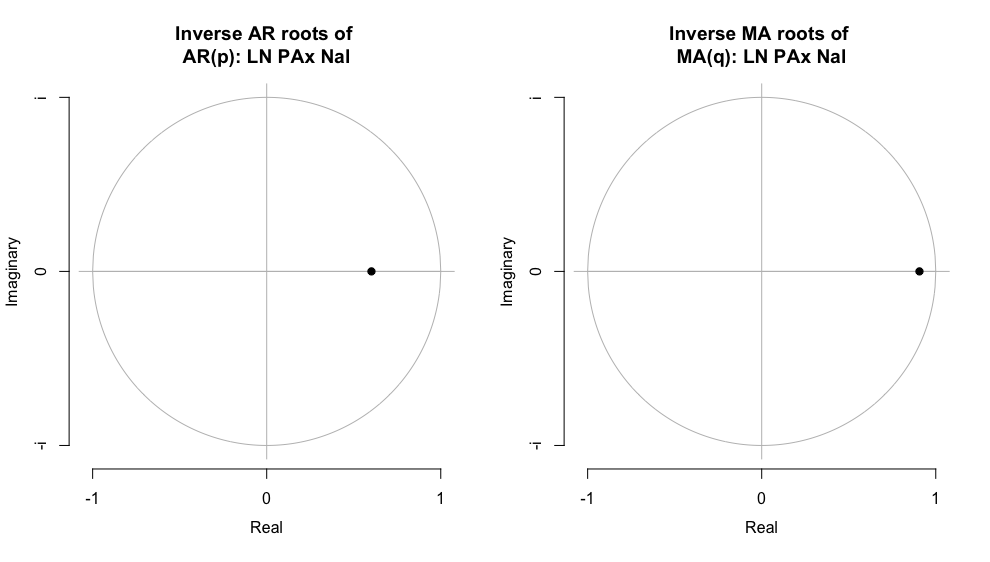
\includegraphics[width = 1.0 \textwidth]{G_Roots_ARMA11}
  \caption{Inveso de las Raíces del polinomio característico de un ARMA(1,1)}
  \label{G_Roots_ARMA11}
\end{figure}

\begin{figure}
\centering
    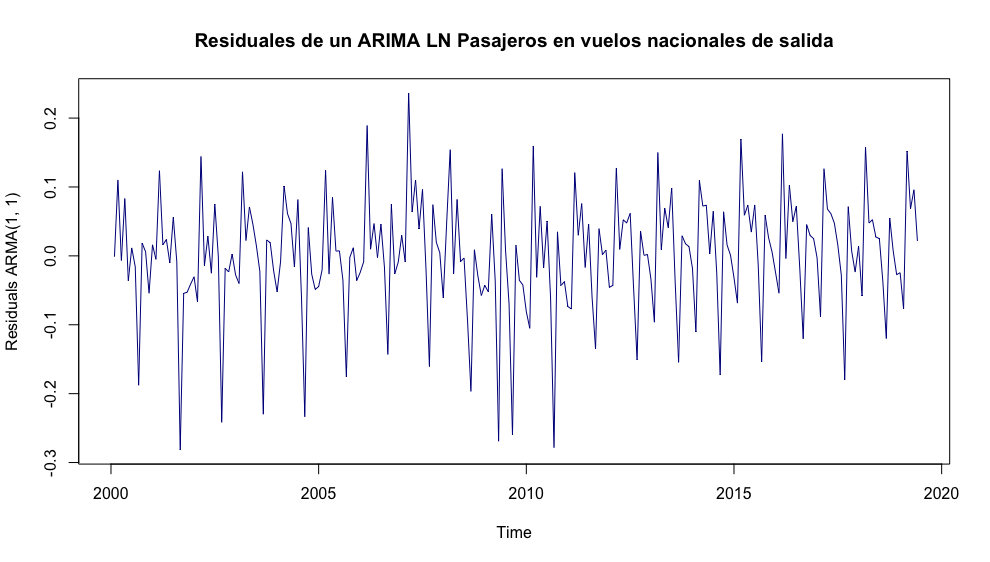
\includegraphics[width = 1.0 \textwidth]{G_Residuals_ARMA11}
    \caption{Residuales de un $ARMA(1, 1)$ de la serie $DLPaxNal_t$}
    \label{G_Residuals_ARMA11}
\end{figure}

En lo que resta de este capítulo, utilizaremos la serie en diferencias
logarítmicas de los pasajeros en vuelos nacionales de salida,
\(DLPaxNal_t\), para discutir los ejemplos que ilustran cada uno de los
puntos teóricos que a continuación exponemos.

\hypertarget{funciuxf3n-de-autocorrelaciuxf3n-parcial}{%
\subsection{Función de Autocorrelación
Parcial}\label{funciuxf3n-de-autocorrelaciuxf3n-parcial}}

Ahora introduciremos el concepto de Función de Autocorrelación Parcial
(PACF, por sus siglas en inglés). Primero, dadas las condiciones de
estabilidad y de convergencia, si suponemos que un proceso AR, MA, ARMA
o ARIMA tienen toda la información de los rezagos de la serie en
conjunto y toda la información de los promedio móviles del término de
error, resulta importante construir una métrica para distinguir el
efecto de \(X_{t - \tau}\) o el efecto de \(U_{t - \tau}\) (para
cualquier \(\tau\)) sobre \(X_t\) de forma individual.

La idea es construir una métrica de la correlación que existe entre las
diferentes varibles aleatorias, si para tal efecto se ha controlado el
efecto del resto de la información. Así, podemos definir la ecuación que
puede responder a este planteamiento como:

\begin{equation}\protect\hypertarget{eq-PACF_Eq}{}{
X_t = \phi_{k1} X_{t-1} + \phi_{k2} X_{t-2} + \ldots + \phi_{kk} X_{t-k} + U_t
}\label{eq-PACF_Eq}\end{equation}

Donde \(\phi_{ki}\) es el coeficiente de la variable dada con el rezago
\(i\) si el proceso tiene un órden \(k\). Así, los coeficientes
\(\phi_{kk}\) son los coeficientes de la autocorrelación parcial
(considerando un proceso AR(k)). Observemos que la autocorrelaicón
parcial mide la correlación entre \(X_t\) y \(X_{t-k}\) que se mantiene
cuando el efecto de las variables \(X_{t-1}\), \(X_{t-2}\), \(\ldots\) y
\(X_{t-k-1}\) en \(X_{t}\) y \(X_{t-k}\) ha sido eliminado.

Dada la expresión considerada en la ecuación (\ref{PACF_Eq}), podemos
resolver el problema de establecer el valor de cada \(\phi_{ki}\)
mediante la solución del sistema que se representa en lo siguiente:

\[
    \left[ 
    \begin{array}{c}
        \rho(1) \\
        \rho(2) \\
        \vdots \\
        \rho(k)
    \end{array} 
    \right]
    = 
    \left[ 
    \begin{array}{c c c c}
        1 & \rho(1) & \ldots & \rho(k - 1)\\
        \rho(1) & 1 & \ldots & \rho(k - 2)\\
        \rho(2) & \rho(1) & \ldots & \rho(k - 3)\\
        \vdots & \vdots & \ldots & \vdots\\
        \rho(k - 1) & \rho(k - 2) & \ldots & 1\\
    \end{array} 
    \right]
    \left[ 
    \begin{array}{c}
        \phi_{k1} \\
        \phi_{k2} \\
        \phi_{k3} \\
        \vdots \\
        \phi_{kk} \\
    \end{array} 
    \right]
\]

Del cual se puede derivar una solución, resoviendo por el método de
cramer, o cualquier otro método que consideremos y que permita calcular
la solución de sistemas de ecuaciones.

Posterior al análisis analítico platearemos un enfoque para interpretar
las funciones de autocorrelación y autocorrelación parcial. Este enfoque
pretende aportar al principio de parcimonia, en el cual podemos
identificar el número de parámetros que posiblemente puede describir
mejor a la serie en un modelo ARMA(p, q).

En el Cuadro \ref{ACF_PACF} se muestra un resumen de las caranterísticas
que debemos observar para determinar el número de parámetros de cada uno
de los componentes AR y MA. Lo anterior por observación de las funciones
de autocorrelación y autocorrelación parcial. Este enfoque no es el más
formal, más adelante implemtaremos uno más formal y que puede ser más
claro de cómo determinar el númeto de parámetros.

\begin{table}
\centering
\begin{tabular}{| c | c | c |}
    \hline
    Modelo  & Función de Autocorrelación & Función de Autocorrelación \\
     si: &   & Parcial \\
    \hline
    MA(q) & Rompimienttos en la función & No hay rompimientos \\
    AR(p) & No hay rompimientos & Rompimienttos en la función \\
    \hline
    \end{tabular}
\caption{Relación entre la Función de Autocorrelación y la Función de Autocorrelación Parcial de una serie $X_t$.}
\label{ACF_PACF}
\end{table}

Continuando con el ejemplo en la Figura (\ref{G_ACF_PACF}) mostramos
tanto la Función de Autocorrelación como la Función de Autocorrelación
Parcial. En esta identificamos que ambas gráficas muestran que el modelo
que explica a la variable \(DLPaxNal_t\) tiene tanto componentes AR como
MA. Sin embargo, dado lo errático del comportamiento de ambas funciones,
resulta complicado determinar cuál sería un buen número de parametros
\(p\) y \(q\) a considerar en el \(ARMA(p,q)\). Por esta razón a
continuación platearemos algunas pruebas más formales para determinar
dichos parámetros.

\begin{figure}
  \centering
    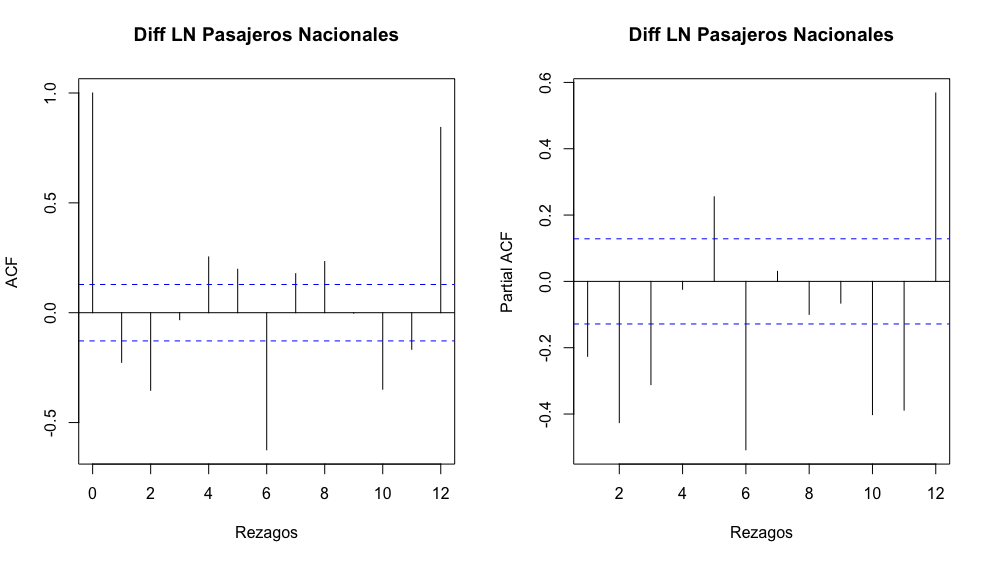
\includegraphics[width = 1.0 \textwidth]{G_ACF_PACF}
  \caption{Función de Autocorrelación y la Función de Autocorrelación Parcial de una serie $DLPaxNal_t$.}
  \label{G_ACF_PACF}
\end{figure}

\hypertarget{selecciuxf3n-de-las-constantes-p-q-d-en-un-arp-un-maq-un-armap-q-o-un-arimap-d-q}{%
\subsection{Selección de las constantes p, q, d en un AR(p), un MA(q),
un ARMA(p, q) o un ARIMA(p, d,
q)}\label{selecciuxf3n-de-las-constantes-p-q-d-en-un-arp-un-maq-un-armap-q-o-un-arimap-d-q}}

Respecto de cómo estimar un proceso ARMA(p, q) --en general utilizaremos
este modelo para discutir, pero lo planteado en esta sección es
igualmente aplicable en cualquier otro caso como aquellos modelos que
incluyen variables exogénas-- existen diversas formas de estimar los
paramétros \(a_i\) y \(b_i\): i) por máxima verosimilitd y ii) por
mínimos cuadrados órdinarios. El primer caso requiere que conozcamos la
distribución del proceso aleatorio \(U_t\). El segundo, por el
contrario, no requiere el mismo supuesto. No obstante, para el curso
utilizaremos el método de máxima verosimilitud.

Otra duda que debe quedar hasta el momento es ¿cómo determinar el orden
\(p\) y \(q\) del proceso ARMA(p, q)? La manera más convencional y
formal que existe para tal efecto es utilizar los criterios de
información. Así, el orden se elije de acuerdo a aquel críterio de
información que resulta ser el mínimo. En el caso de \(d\) se selecciona
revisando la gráfica que parezca más estacionaria--más adelante
mostraremos un proceso más formal para su selección.

Los criterios de información más comunes son los siguientes:

\begin{enumerate}
\def\labelenumi{\arabic{enumi}.}
\tightlist
\item
  FPE (Final Prediction Error):
\end{enumerate}

\[
FPE = \frac{T+m}{T-m}\frac{1}{T}\sum_{t=1}^{T} \left( \hat{U}_t^{(p)} \right) ^2
\] 2. Akaike:

\[
AIC = ln \left[ \frac{1}{T} \sum_{t=1}^{T} \left( \hat{U}_t^{(p)} \right) ^2 \right] + m \frac{2}{T}
\] 3. Schwarz:

\[
SC = ln \left[ \frac{1}{T} \sum_{t=1}^{T} \left( \hat{U}_t^{(p)} \right) ^2 \right] + m \frac{ln(T)}{T}
\] 4. Hannan - Quinn:

\[
HQ = ln \left[ \frac{1}{T} \sum_{t=1}^{T} \left( \hat{U}_t^{(p)} \right) ^2 \right] + m \frac{2 ln(ln(T))}{T}
\]

Donde \(\hat{U}_t^{(p)}\) son los residuales estimados mediante un
proceso ARIMA y \(m\) es el número de parametros estimados:
\(m = p + q + 0 + 1\) (ya que asumimos que \(d = 0\)). Una propiedad que
no se debe perder de vista es que los criterios de información cumplen
la siguiente relación:

\[
orden(SC) \leq orden(HQ) \leq orden(AIC)
\]

Por esta razón, durante el curso solo utilizaremos el criterio se Akaike
para determinar el orden óptimo del proceso ARMA, ya que ello garantiza
el orden más grande posible.

Ahora veamos un ejemplo de estimación del número de rezagos optimo de un
\(ARMA(p, q)\). Retomemos la serie en diferencias logarítmicas de los
pasajeros en vuelos nacionales de salidas, pero ahora incluiremos la
variables exógenas de dummies estacionales: enero, febrero, julio y
diciembre.

Como mencionamos, las gráficas de las funciones de autocorrelación
permiten observar el valor de la correlación existente entre la variable
en el momento \(t\) con cada uno de los rezagos. Incluso la Función de
Autocorrelación Parcial puede ayudar a determinar el número máximo de
rezagos que se debe incluir en el proceso \(AR(p)\). No obstante, una
métrica más formal es el uso de los criterios de información. En nuestro
caso, dado lo discutido, sólo utilizareemos el criterio de Akaike.

Al respecto, en el Cuadro (\ref{Selec_ARMApq}) reportamos el criterio de
Akaike que resultan de aplicar dicho criterio a los residuales
resultantes de cada combinación de procesos \(ARMA(p, q)\). La forma de
escoger será aquel modelo que reporta el criterio de Akaike menor. En la
cuarta columna de la tabla se señala el valor del criterio de
información que resulta ser el mínimo de todos los posibles.

\begin{table}
\centering
\begin{tabular}{|c | c | c | c | c |}
\hline
    Modelo & AR(p) & MA(p) & Akaike (AIC) & Óptimo \\
\hline
    1 & 1 & 1 & -475.1190 &  \\
    2 & 1 & 2 & -473.4397 &  \\
    3 & 1 & 3 & -483.1239 &  \\
    4 & 1 & 4 & -482.4932 &  \\
    5 & 1 & 5 & -506.9880 &  \\
    6 & 1 & 6 & -533.9411 &  \\
    7 & 2 & 1 & -473.4758 &  \\
    $\vdots$ & $\vdots$ & $\vdots$ & $\vdots$ & $\vdots$ \\
    24 & 4 & 6 & -752.8996 & * \\
    $\vdots$ & $\vdots$ & $\vdots$ & $\vdots$ & $\vdots$ \\
    36 & 6 & 6 & -752.2632 &  \\
\hline
\end{tabular}
\caption{Criterio de Akike para diferentes modelos $ARMA(p, q)$ de la serie $DLPaxNal_t$.}
\label{Selec_ARMApq}
\end{table}

El Cuadro (\ref{Selec_ARMApq}) reporta los resultados para 36 diferentes
modelos, todos incluyen variables exogenas. Como resultado del análisis
concluimos que el modelo más adecuado es el 24, el cual considera un
\(ARMA(4, 6)\), con variables dummies para controlar la estacionalidad
de los meses de enero, febrero, julio y diciembre. En el Cuadro
(\ref{Result_ARMApq}) mostramos los resutados del modelo.

No obstante, una inspección de los residuales del modelo nos permite
sospechar que requiere de incluir un par de dummies más. Ambas,
asociadas con la caída del transporte aéreo en 2009, principalmente
asociado con la crisis mundial de ese año. La Figura
(\ref{G_Residuals_ARMA46}) muestra los residuales mencionados.

\begin{figure}
  \centering
    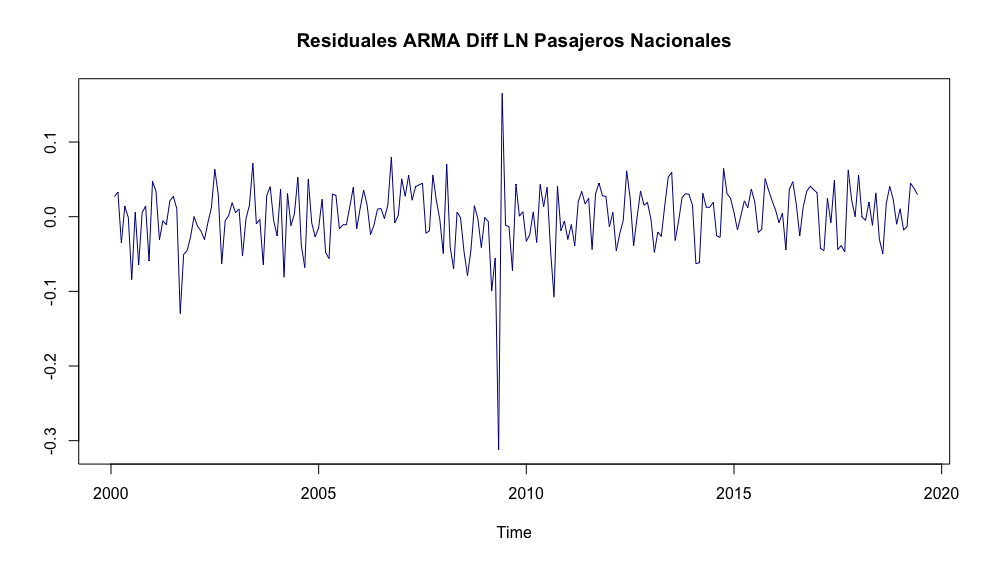
\includegraphics[width = 1.0 \textwidth]{G_Residuals_ARMA46}
  \caption{Residuales del ARMA(4, 6) de una serie $DLPaxNal_t$.}
  \label{G_Residuals_ARMA46}
\end{figure}

Una vez incluidas dos dummies más para mayo y junio de 2009, analizamos
un total de 36 modelos ARMA y determinamos que el orden que minimizza el
criterio de Akaike es un \(ARMA(4, 6)\). El Cuadro (\ref{Result_ARMApq})
muestra los resultados para este nuevo modelo. No lo motramos en esta
sección, pero ambos modelos reportados tienen raices de sus respectivos
polinomios característicos menores a 1 en valor absoluto. En la Figura
\ref{G_Residuals_ARMA46_D} mostramos los residuales ahora ajustados por
las dummies de mayo y junio de 2009.

\begin{table}
\centering
\begin{tabular}{|c | c | c | c | c |}
\hline
     & \multicolumn{2}{| c |}{Modelo 1} & \multicolumn{2}{| c |}{Modelo 2} \\
\hline
    Variable & Coeficiente & Error Est. & Coeficiente & Error Est. \\
\hline
    Constante & 0.0134 & 0.0033 & 0.0145 & 0.0029 \\
    $DLPaxNal_{t-1}$ & 0.0004 & 0.0011 & 0.0014 & 0.0016 \\
    $DLPaxNal_{t-2}$ & 0.9997 & 0.0019 & 0.9988 & 0.0024 \\
    $DLPaxNal_{t-3}$ & 0.0001 & 0.0012 & 0.0002 & 0.0014 \\
    $DLPaxNal_{t-4}$ & -0.9997 & 0.0004 & -0.9993 & 0.0009 \\
    $\hat{U}_{t-1}$ & -0.2877 & 0.0670 & -0.1472 & 0.0633 \\
    $\hat{U}_{t-2}$ & -1.2028 & 0.0608 & -1.3323 & 0.0625 \\
    $\hat{U}_{t-3}$ & 0.2302 & 0.0765 & 0.1201 & 0.0756 \\
    $\hat{U}_{t-4}$ & 1.2085 & 0.0645 & 1.3142 & 0.0642 \\
    $\hat{U}_{t-5}$ & -0.2634 & 0.0708 & -0.1034 & 0.0717 \\
    $\hat{U}_{t-6}$ & -0.2171 & 0.0606 & -0.3864 & 0.0657 \\
    $DEne_{t}$ & -0.2904 & 0.0172 & -0.2865 & 0.0156 \\
    $DFeb_{t}$ & -0.1312 & 0.0170 & -0.1273 & 0.0140 \\
    $DJul_{t}$ & 0.3303 & 0.0173 & 0.3164 & 0.0156 \\
    $Dic_{t}$ & -0.0118 & 0.0169 & -0.0138 & 0.0137 \\
    $DMay2009_{t}$ &   &   & -0.3378 & 0.0360 \\
    $DJun2009_{t}$ &   &   & 0.2371 & 0.0359 \\
\hline
    $\hat{\sigma}^2$ & 0.001841 &   & 0.001283 &  \\
    AIC & -752.9 &   & -835.73 &  \\
\hline
    \multicolumn{5}{ l }{Nota: El método de estimación fue máxima verosimilitud.} \\
\end{tabular}
\caption{Criterio de Akike para diferentes modelos ARMA(p, q) de la serie $DLPaxNal_t$.}
\label{Result_ARMApq}
\end{table}

\begin{figure}
  \centering
    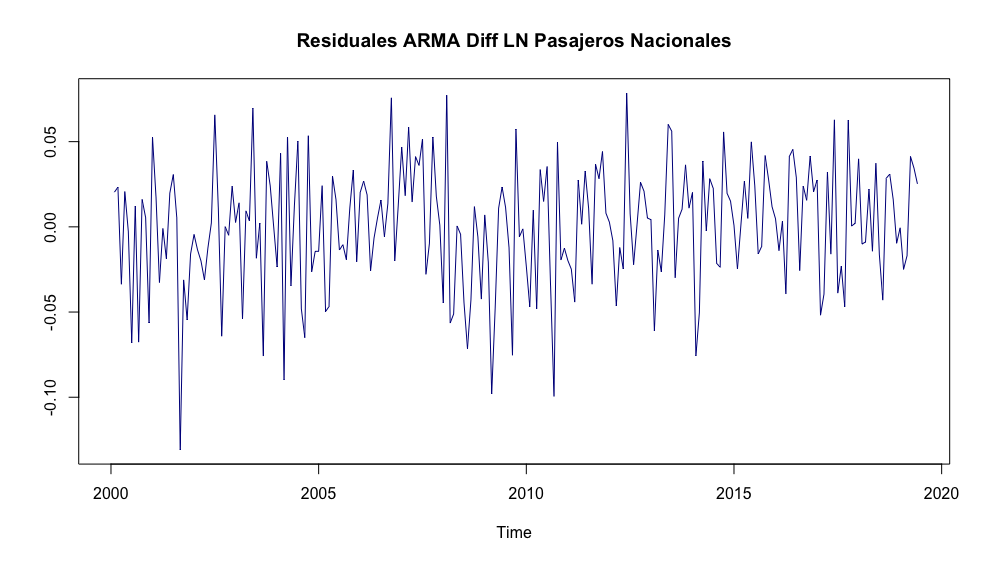
\includegraphics[width = 1.0 \textwidth]{G_Residuals_ARMA46_D}
  \caption{Residuales del ARMA(4, 6) de una serie $DLPaxNal_t$.}
  \label{G_Residuals_ARMA46_D}
\end{figure}

\hypertarget{pronuxf3sticos}{%
\subsection{Pronósticos}\label{pronuxf3sticos}}

Para pronósticar el valor de la serie es necesario determinar cuál es el
valor esperado de la serie en un momento \(t + \tau\) condicional en que
ésta se comporta como un \(AR(p)\), un \(MA(q)\) o un \(ARMA(p, q)\) y a
que los valores antes de \(t\) están dados. Por lo que el pronóstico de
la serie estará dado por una expresión:

\begin{eqnarray}
    \mathbb{E}_t[X_{t+\tau}] = \delta + a_1 \mathbb{E}_t[X_{t+\tau-1}] + a_2 \mathbb{E}_t[X_{t+\tau-2}] + \ldots + + a_p \mathbb{E}_t[X_{t+\tau-p}]
\end{eqnarray} \{\#eq-ARMApq\_For\}

Lo anterior para todo \(\tau = 0, 1, 2, \ldots\) y considerando que los
componentes MA(q) en la eucación (\ref{ARMApq_For}) son cero dado que
para todo valor \(t + \tau\) es cierto que \(\mathbb{E}_t[U_{t+\tau}]\).

Continuando con el ejemplo, en la Figura (\ref{Pax_Nal_f}) mostramos el
resultado del pronóstico de la serie a partir del modelo ARMA(4, 6) que
hemos discutido anteriormente.

\begin{figure}
  \centering
    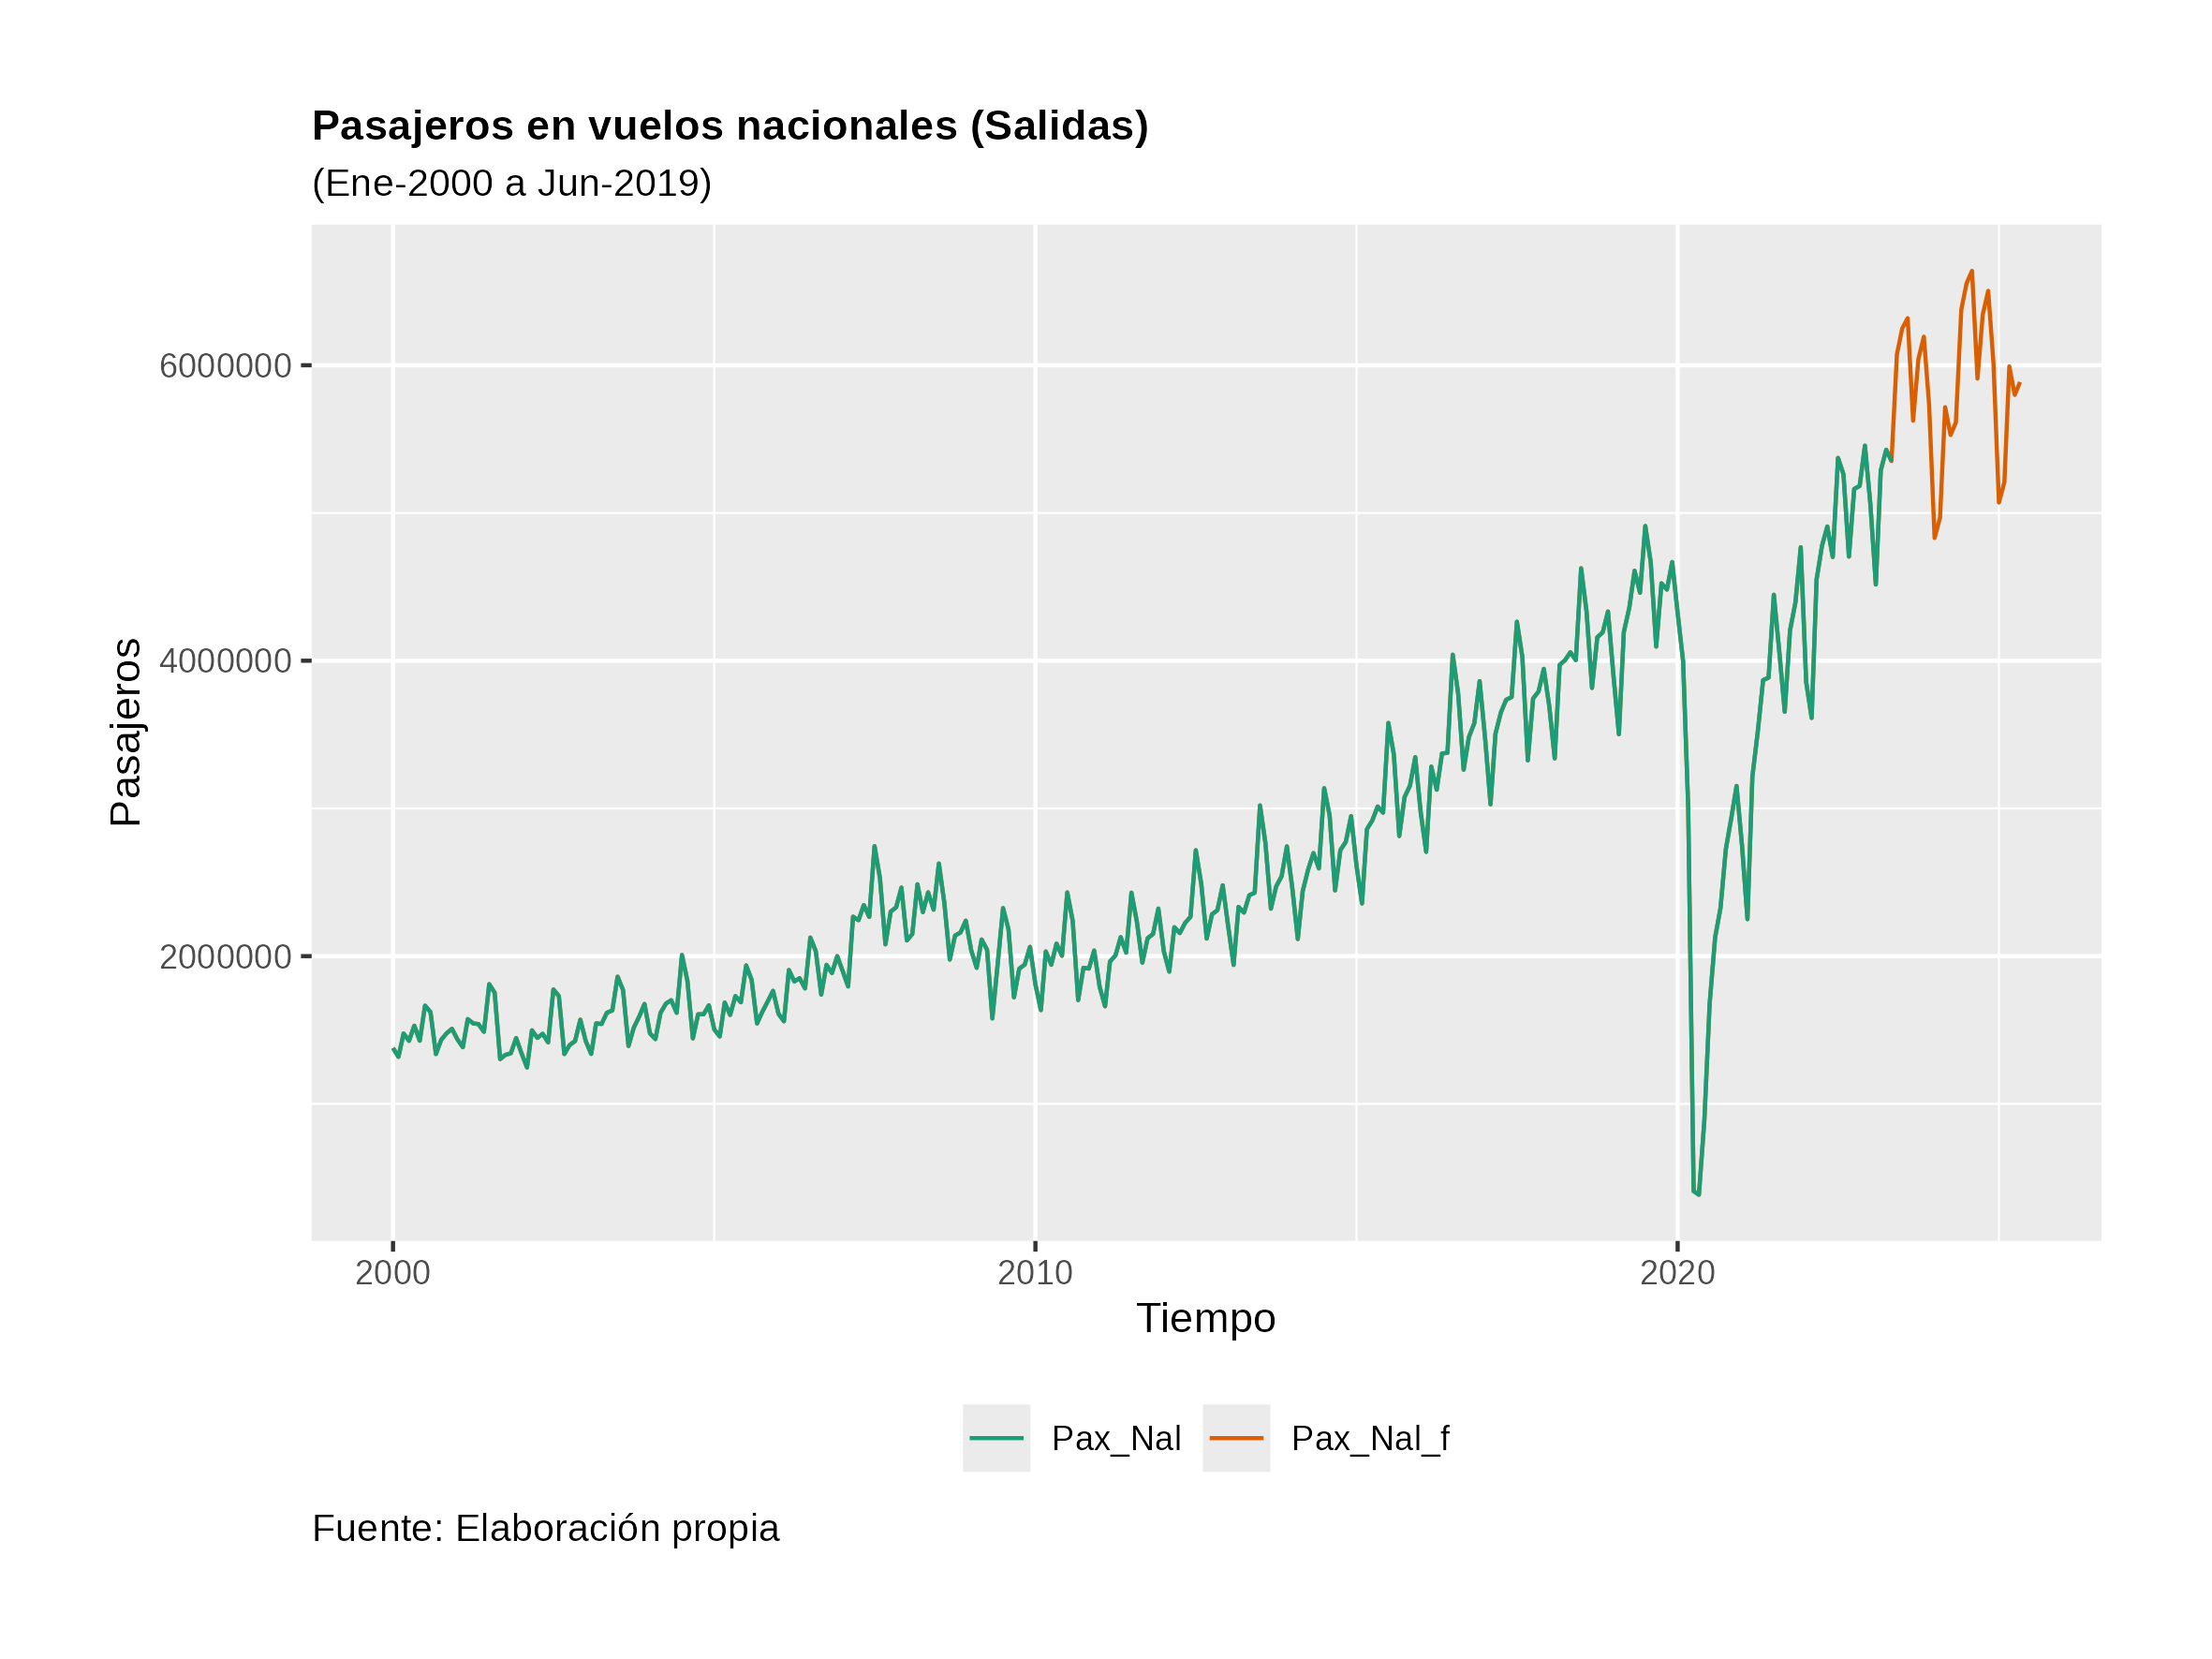
\includegraphics[width = 1.0 \textwidth]{Pax_Nal_f}
  \caption{Pronóstico de la serie $PaxNAl_t$ a partir de una ARMA(4,6) en diferencias logaritmicas.}
  \label{Pax_Nal_f}
\end{figure}


\printbibliography


\end{document}
